We classically simulated the NVQWOA on randomly generated unlabelled graph similarity instances of size $n=8,9,10$. Each size included 30 distinct problem instances, and each was evolved for $p=10$ iterations under hyperparameters optimised for three objective functions. Across all analyses, we observed consistent amplification of optimal and near-optimal solutions, strong correlation between amplification and solution proximity to the optimum, and mixing dynamics that align with theoretical predictions for suitability.

When referring to the hyperparameter optimisation objective functions explained in section \ref{sec:parameters}, we use the acronyms EV for expectation value, OSP for optimal solution probability, and CVaR for conditional value at risk.

\section{Amplification Analysis}
The first analysis aimed to verify that the NVQWOA amplifies the measurement probability of optimal and near-optimal solutions relative to the uniform initial state distribution. 

Figures \ref{fig:similarity dist} and \ref{fig:similarity log dist} show the average probability distributions over the possible similarity scores, using a linear probability scale for Figure \ref{fig:similarity dist} and a log probability scale for \ref{fig:similarity log dist}. The post-amplification distributions are skewed towards higher-similarity solutions compared to the initial distribution.


\begin{figure}[htbp]
    \centering
    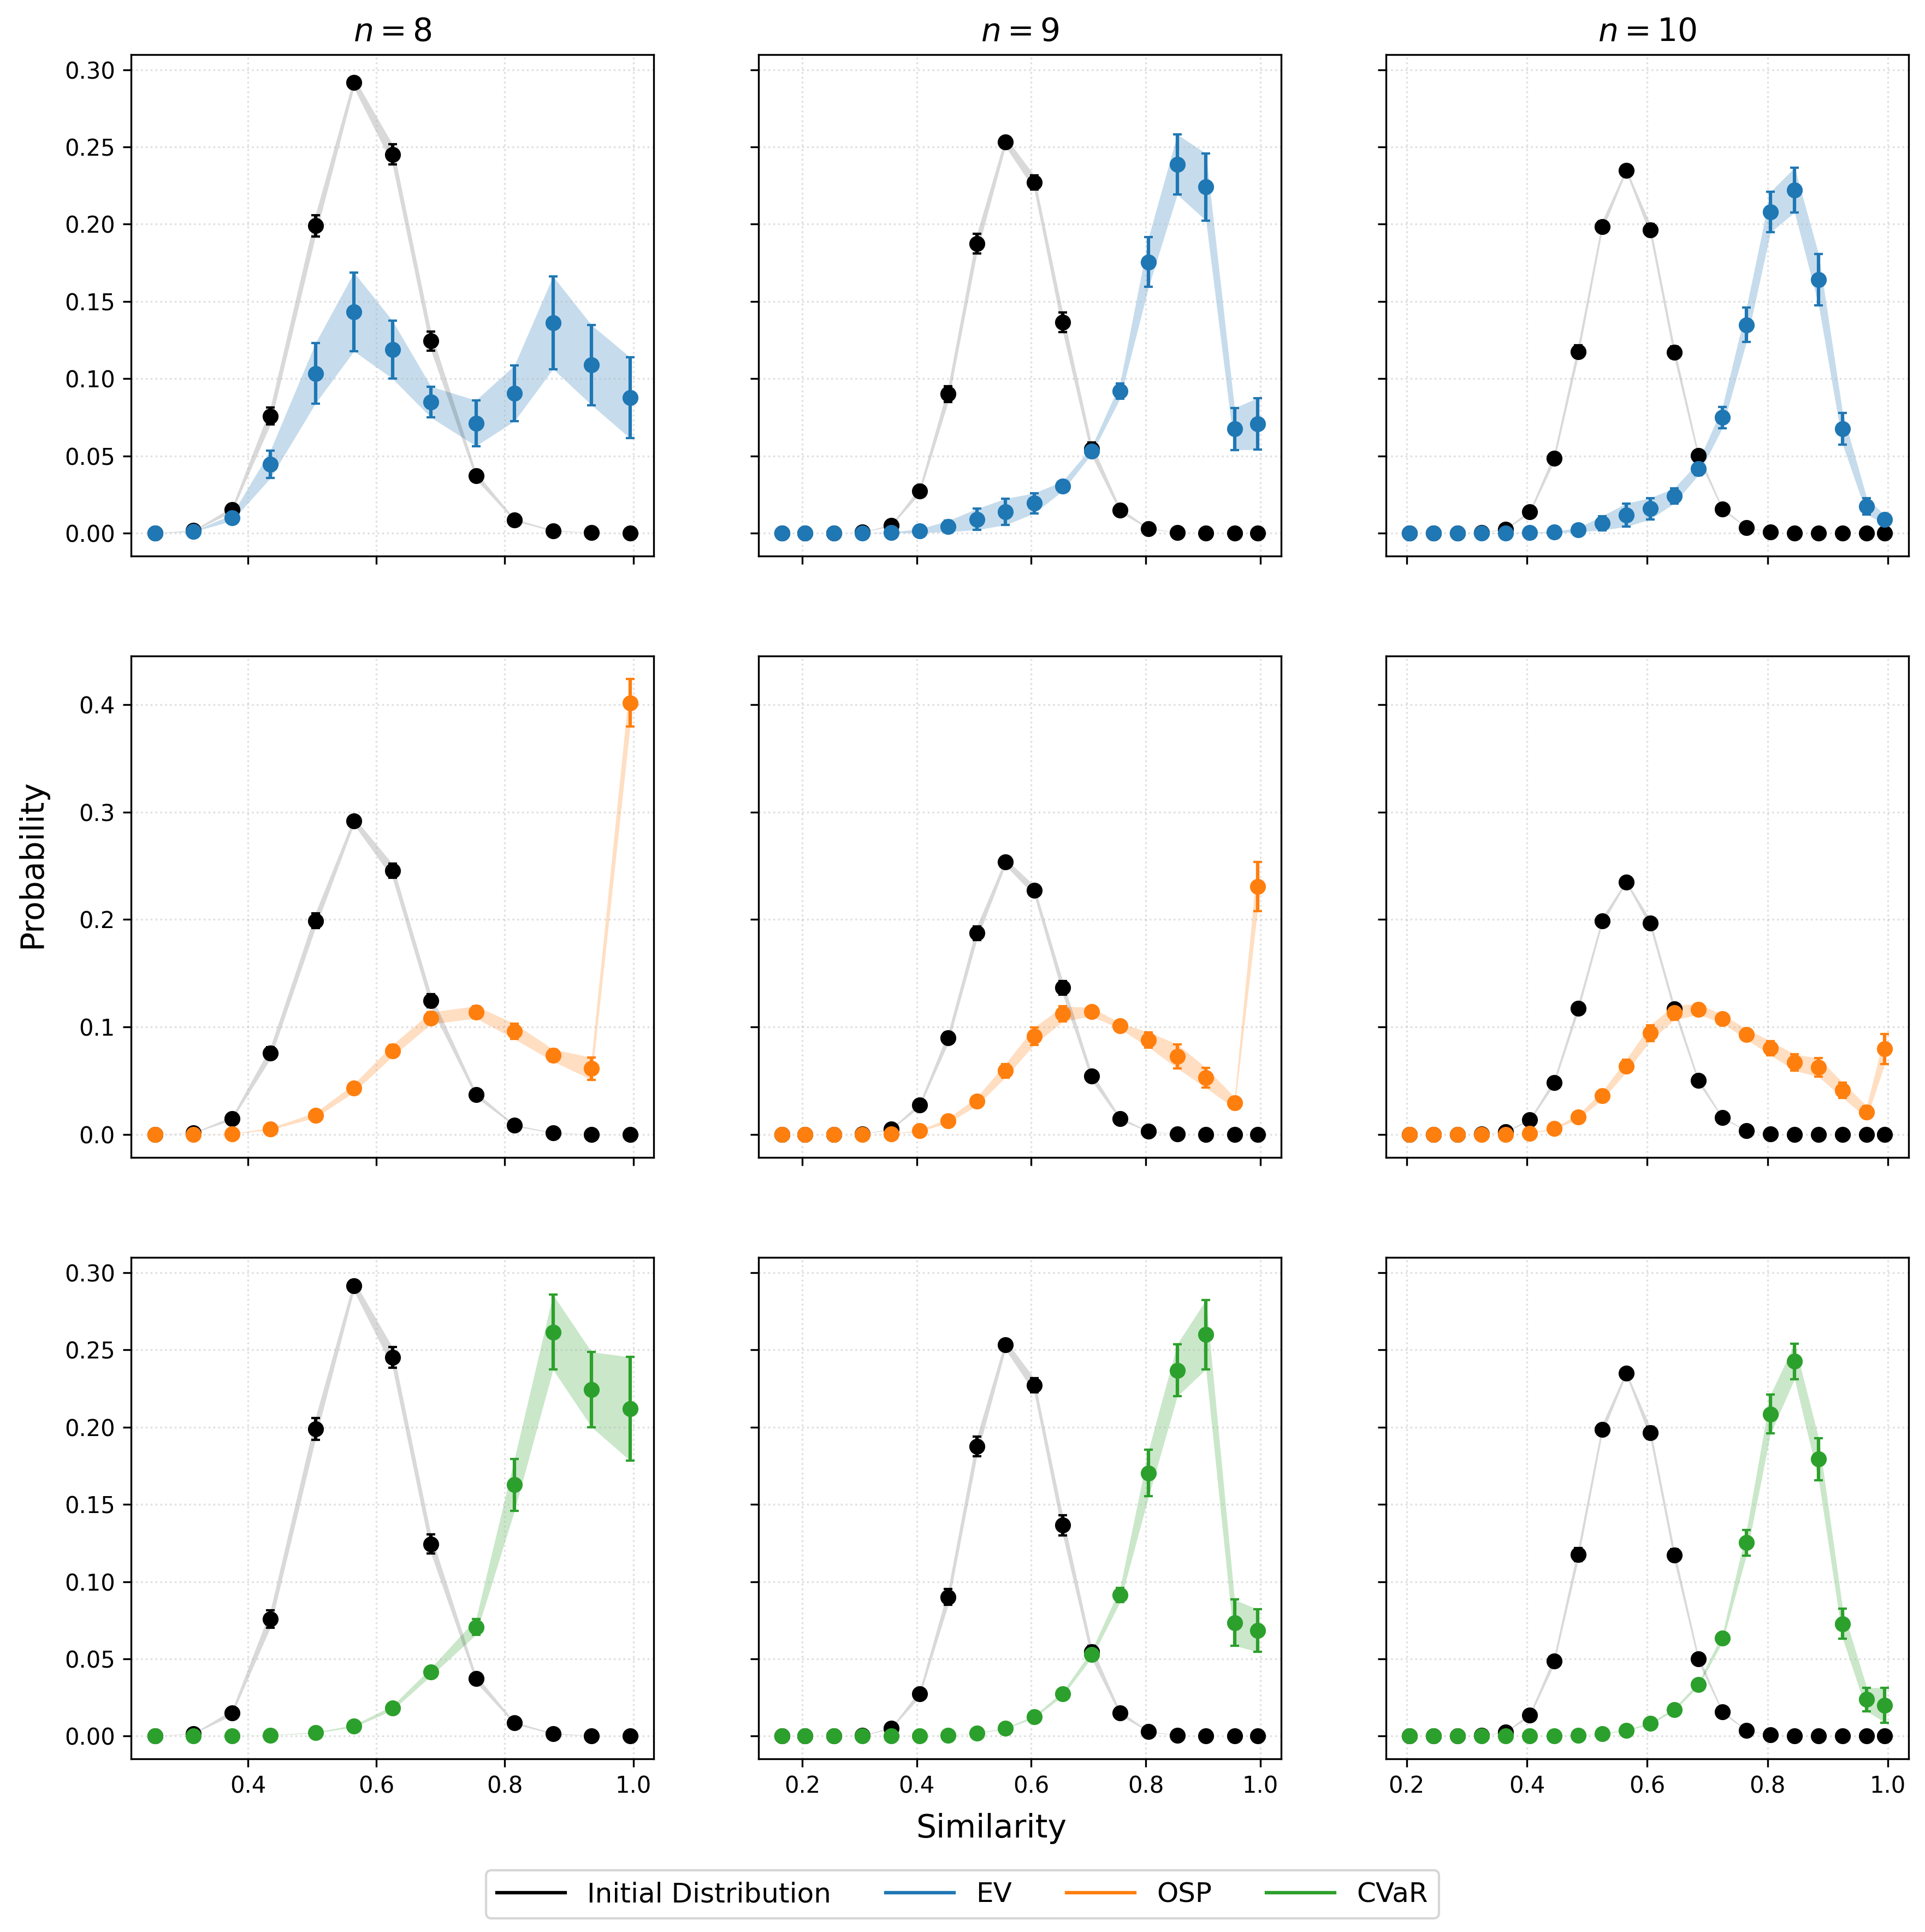
\includegraphics[width=\textwidth]{similarity_distributions_multiple.png} 
    \caption{Probability distributions over the possible similarities.}
    \label{fig:similarity dist}
\end{figure}

\begin{figure}[htbp]
    \centering
    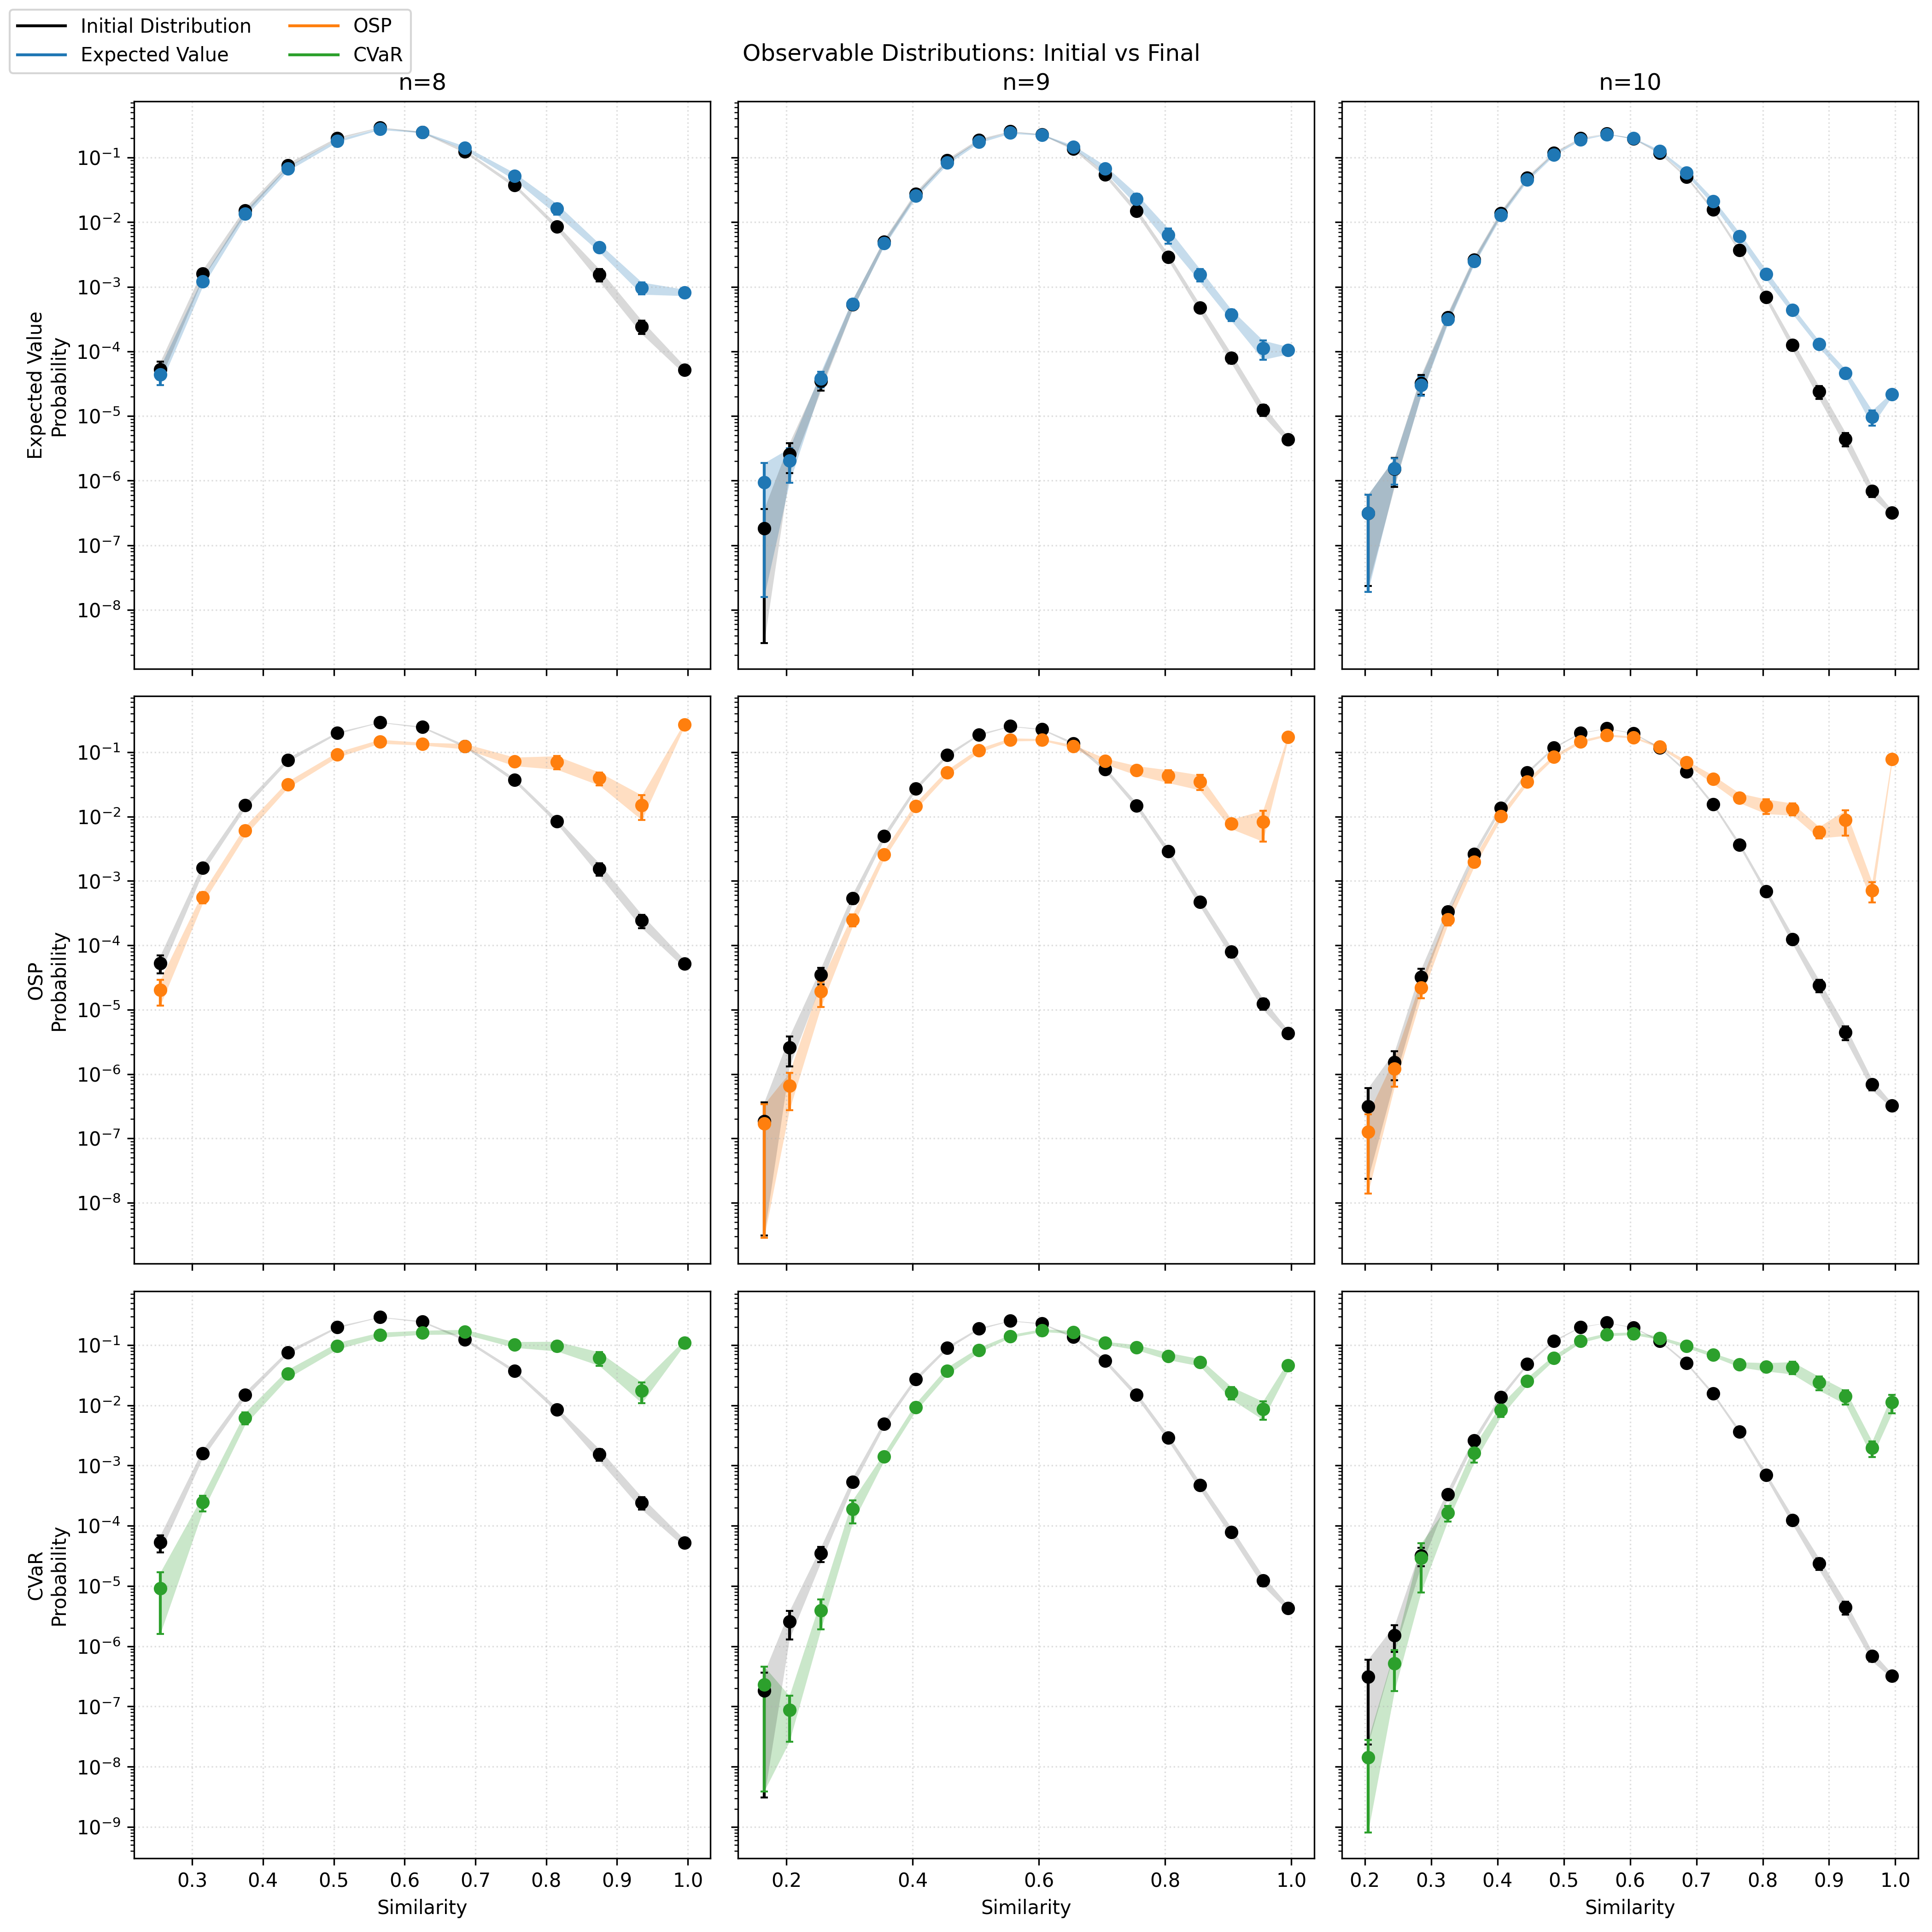
\includegraphics[width=\textwidth]{log_similarity_distributions_multiple.png} 
    \caption{Depicts the same distributions as Fig \ref{fig:similarity dist} with a logarithmic y-axis.}
    \label{fig:similarity log dist}
\end{figure}

Figure \ref{fig:osp} is a boxplot showing the probability of measuring the optimal solution after amplification. The OSP varied significantly across problem instances but consistently improved following NVQWOA evolution. Median OSP values increased by more than an order of magnitude over the initial probability when using EV.

\begin{figure}[htbp]
    \centering
    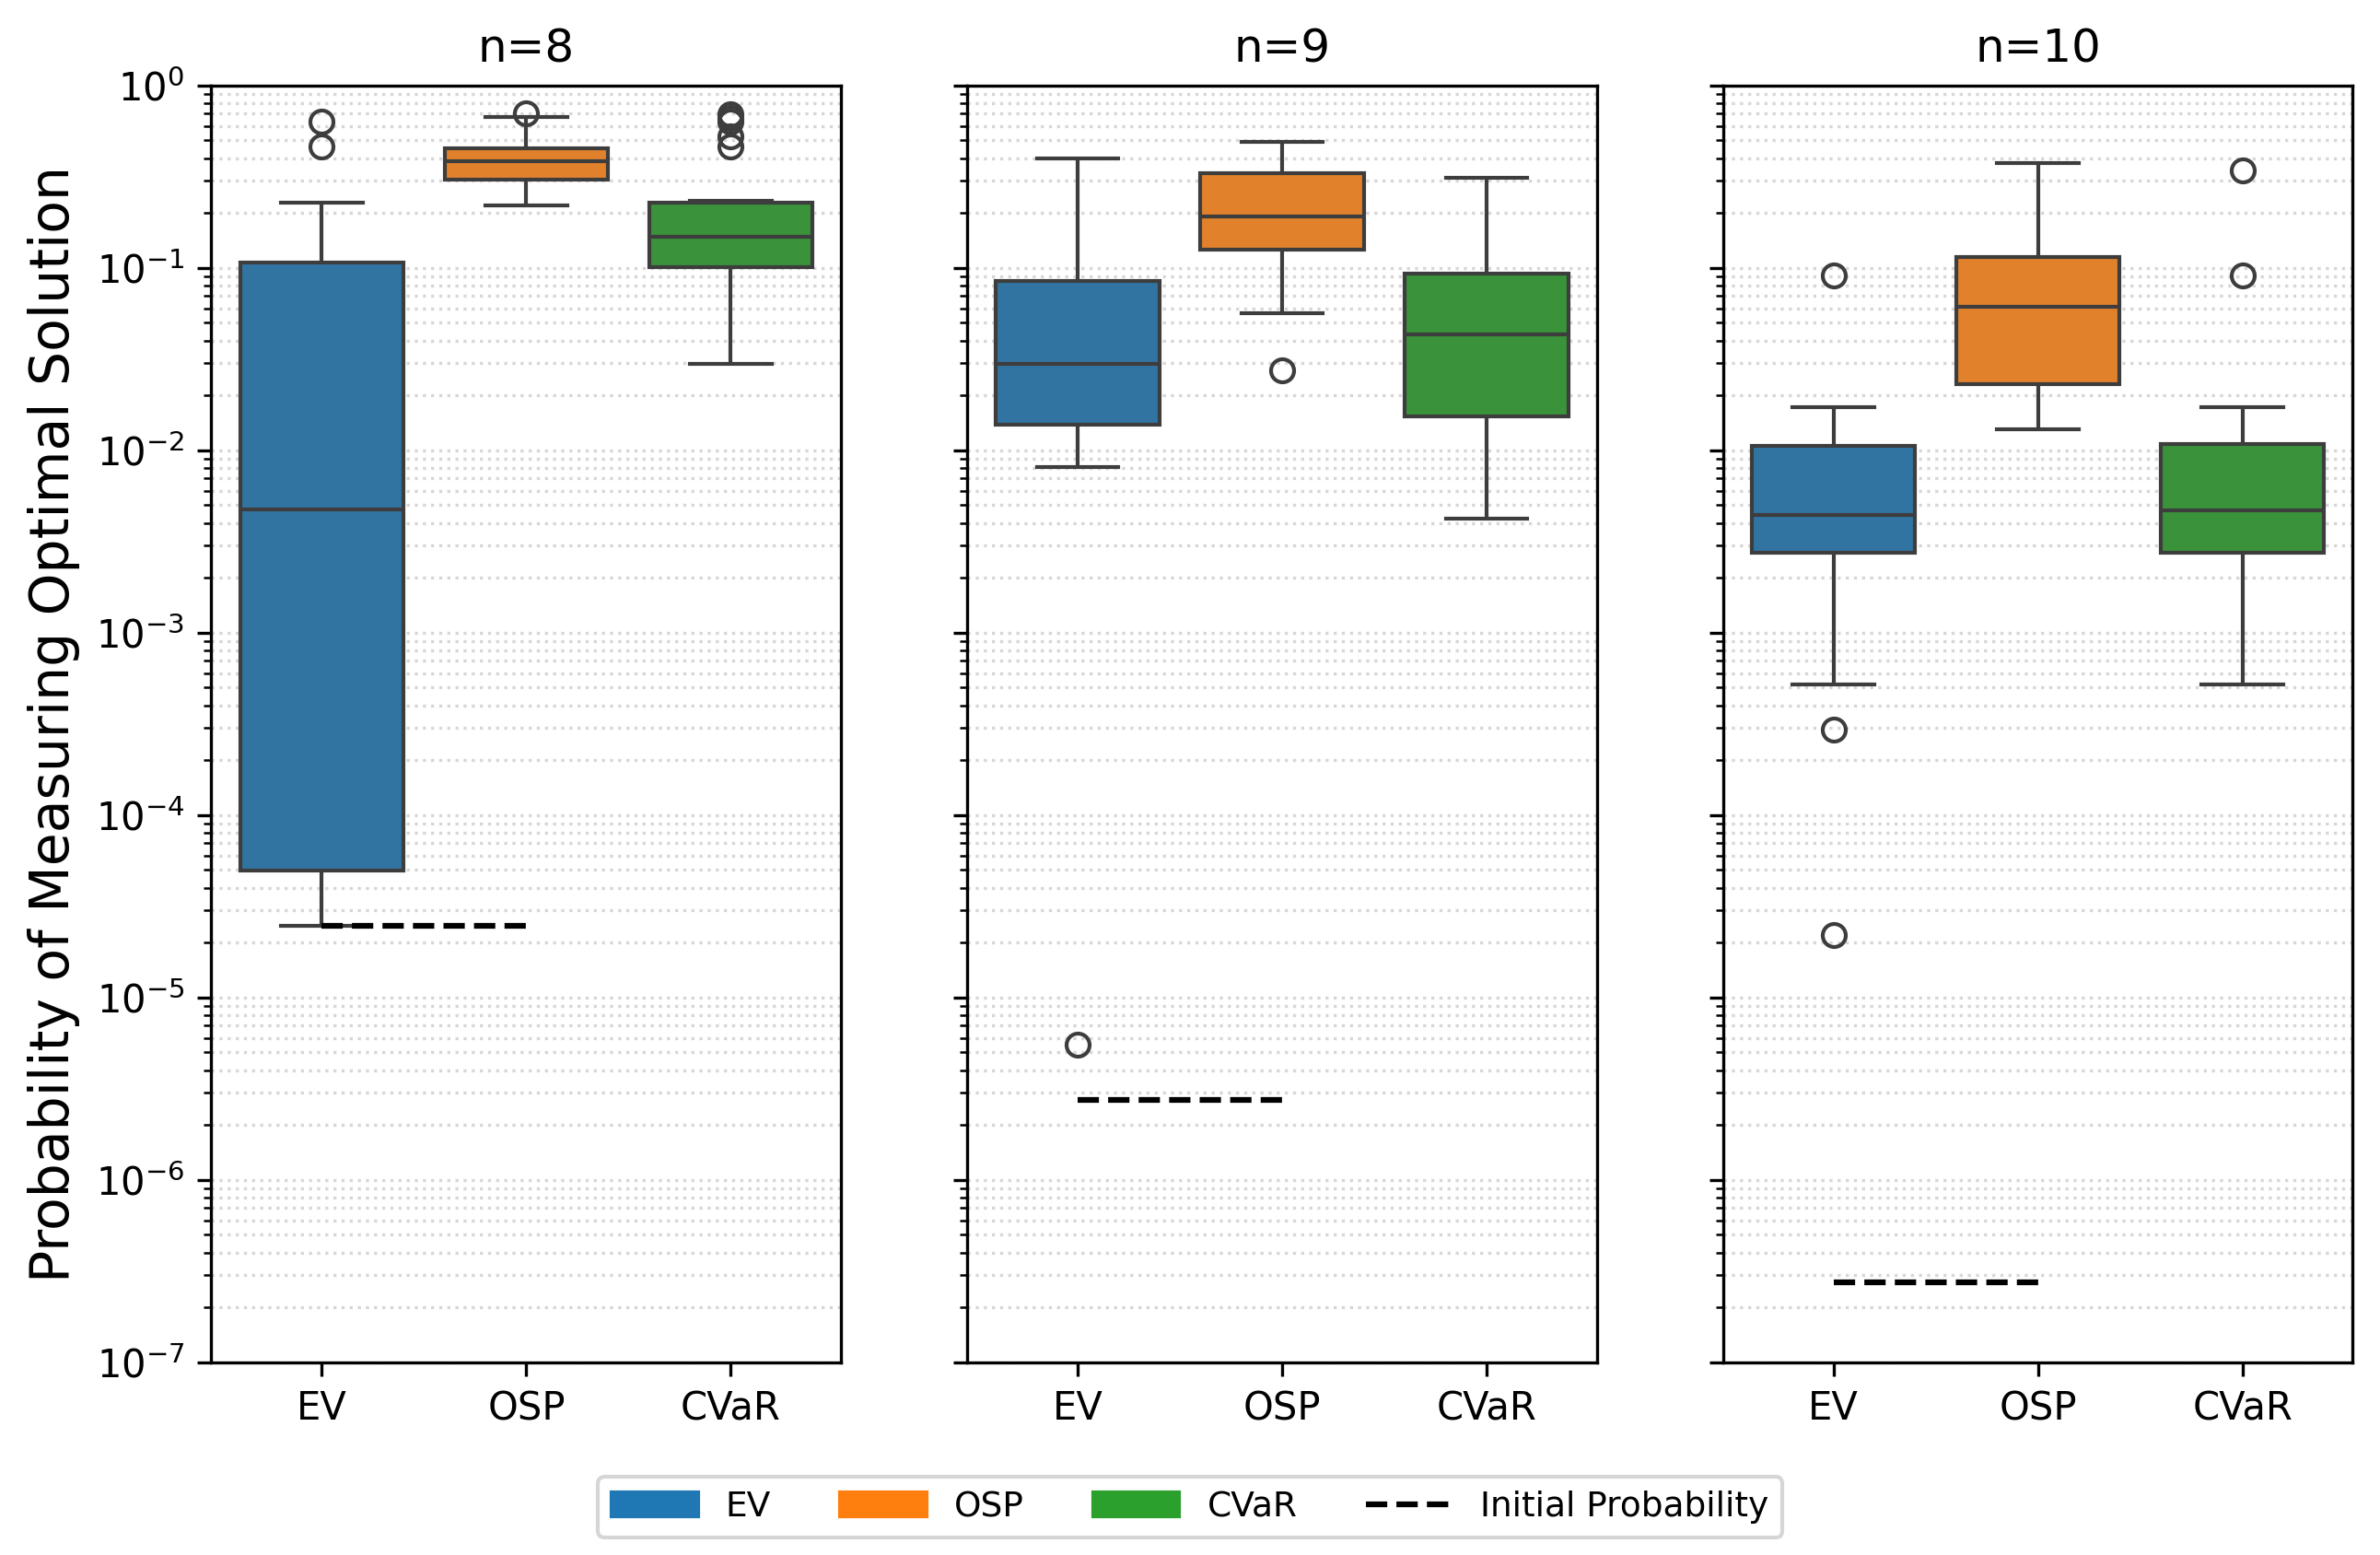
\includegraphics[width=\textwidth]{OSP_boxplot_multiple.png} 
    \caption{Boxplots representing the probability to measure the optimal solution. The average upper bound represents the mean OSP over all problem instances after optimising the hyperparameters to maximise the OSP.}
    \label{fig:osp}
\end{figure}



\section{Hamming Distance Analysis}
We next analysed the Hamming distance between each solution and the optimal solution(s) to determine whether amplification favours solutions close to the optimum in the solution space.

Figure \ref{fig:avg ham} shows the mean Hamming distance before and after amplification for each problem instance.
\begin{figure}[htbp]
     \centering
     \begin{subfigure}{0.45\textwidth}
         \centering
         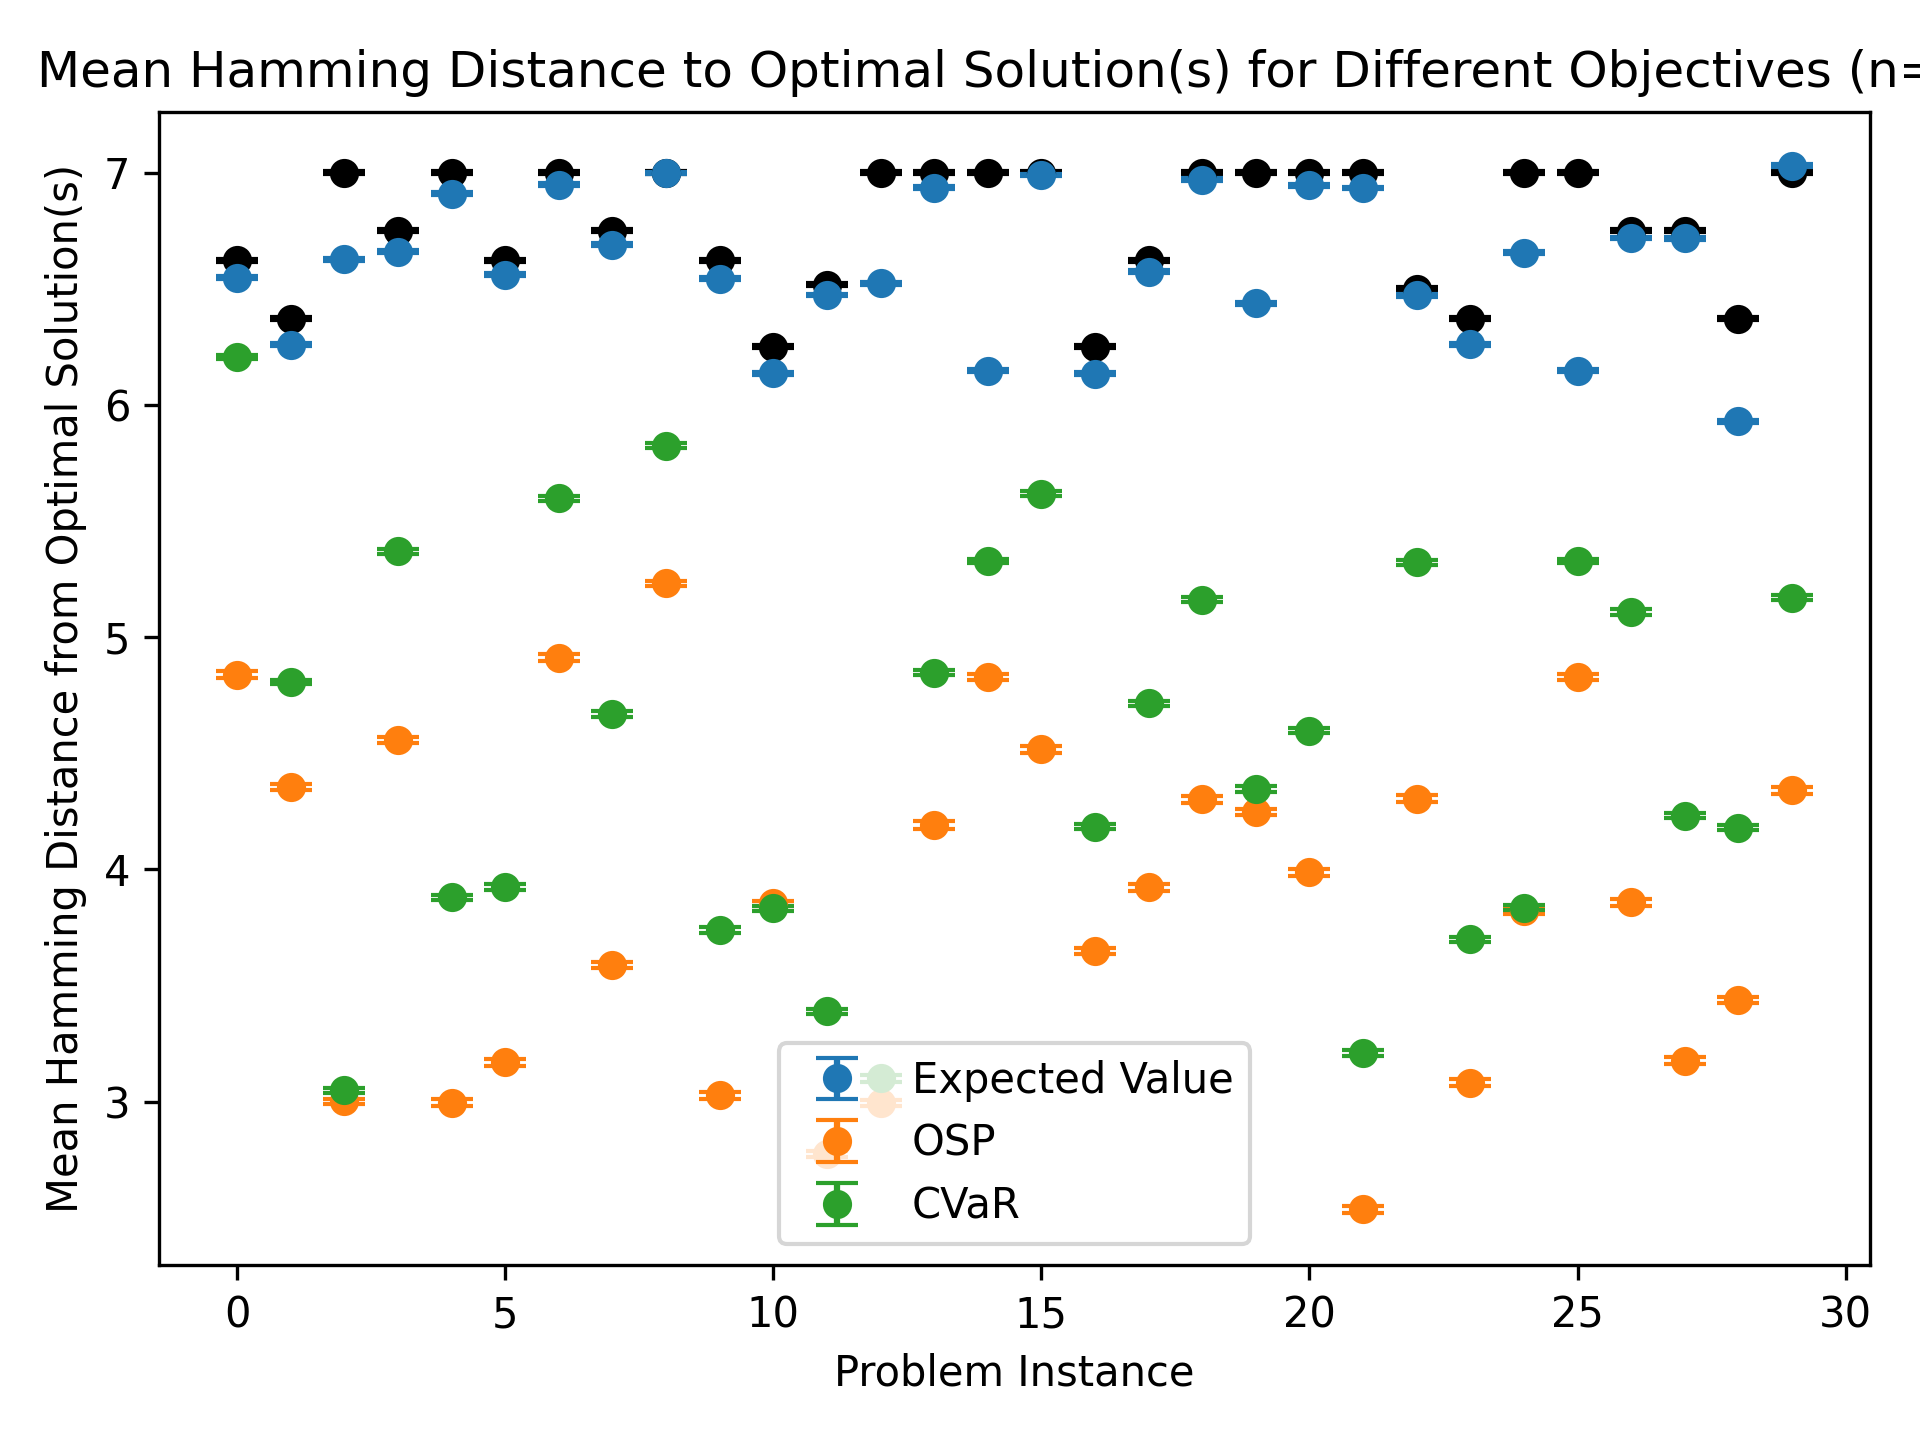
\includegraphics[width=\textwidth]{n=8_avg_hamming_distance_each_instance.png}
         \caption{$n=8$}
         \label{fig:avg ham 8}
     \end{subfigure}
     \hfill
     \begin{subfigure}{0.45\textwidth}
         \centering
         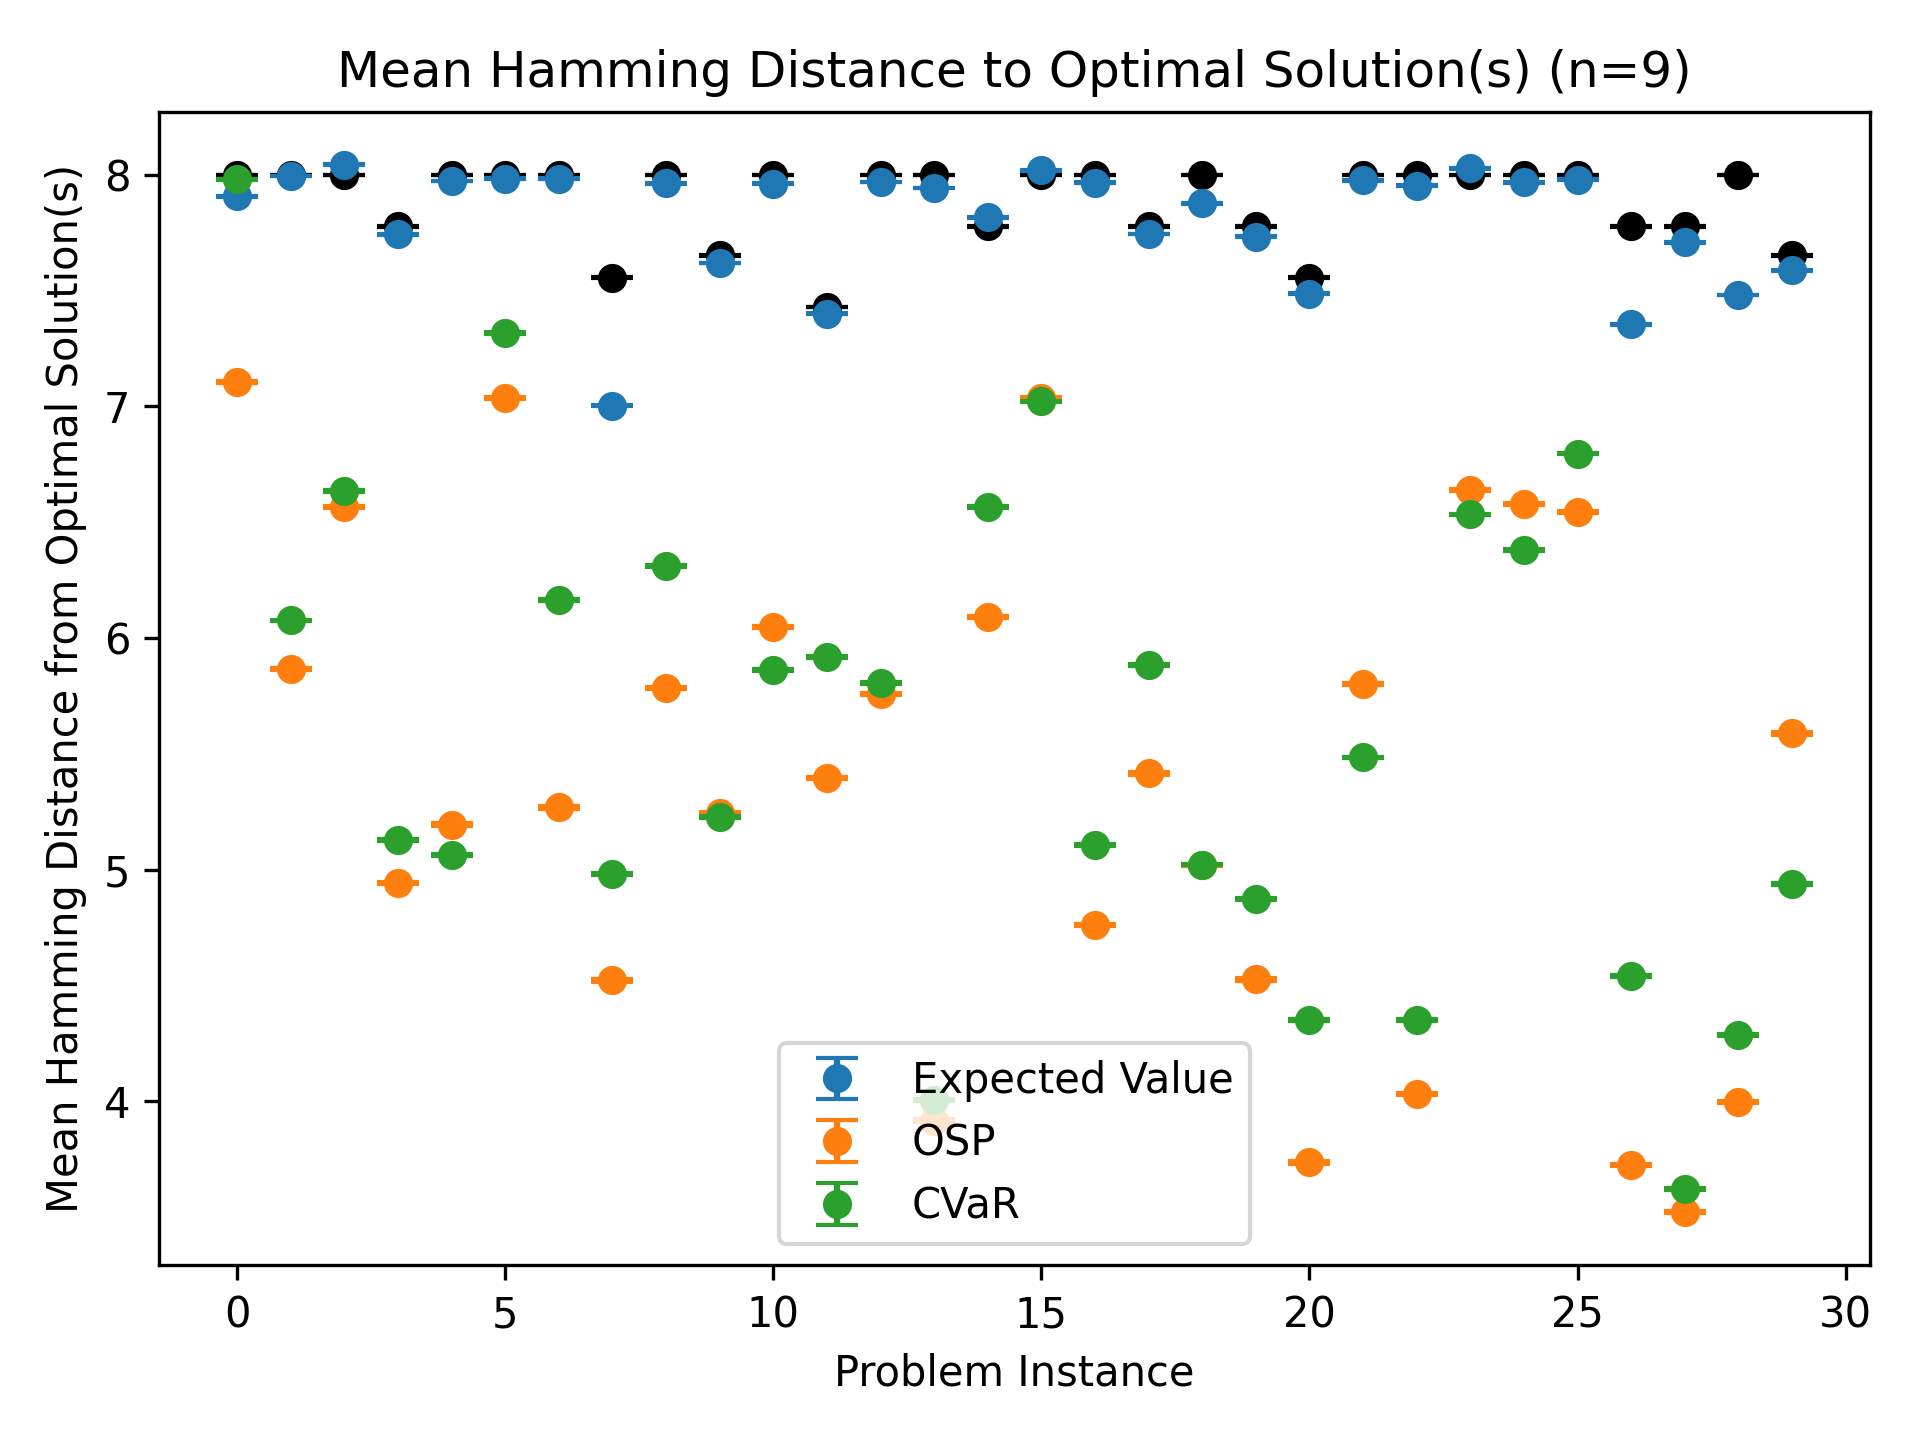
\includegraphics[width=\textwidth]{n=9_avg_hamming_distance_each_instance.png}
         \caption{$n=9$}
         \label{fig:avg ham 9}
     \end{subfigure}
     \hfill
     \begin{subfigure}{\textwidth}
         \centering
         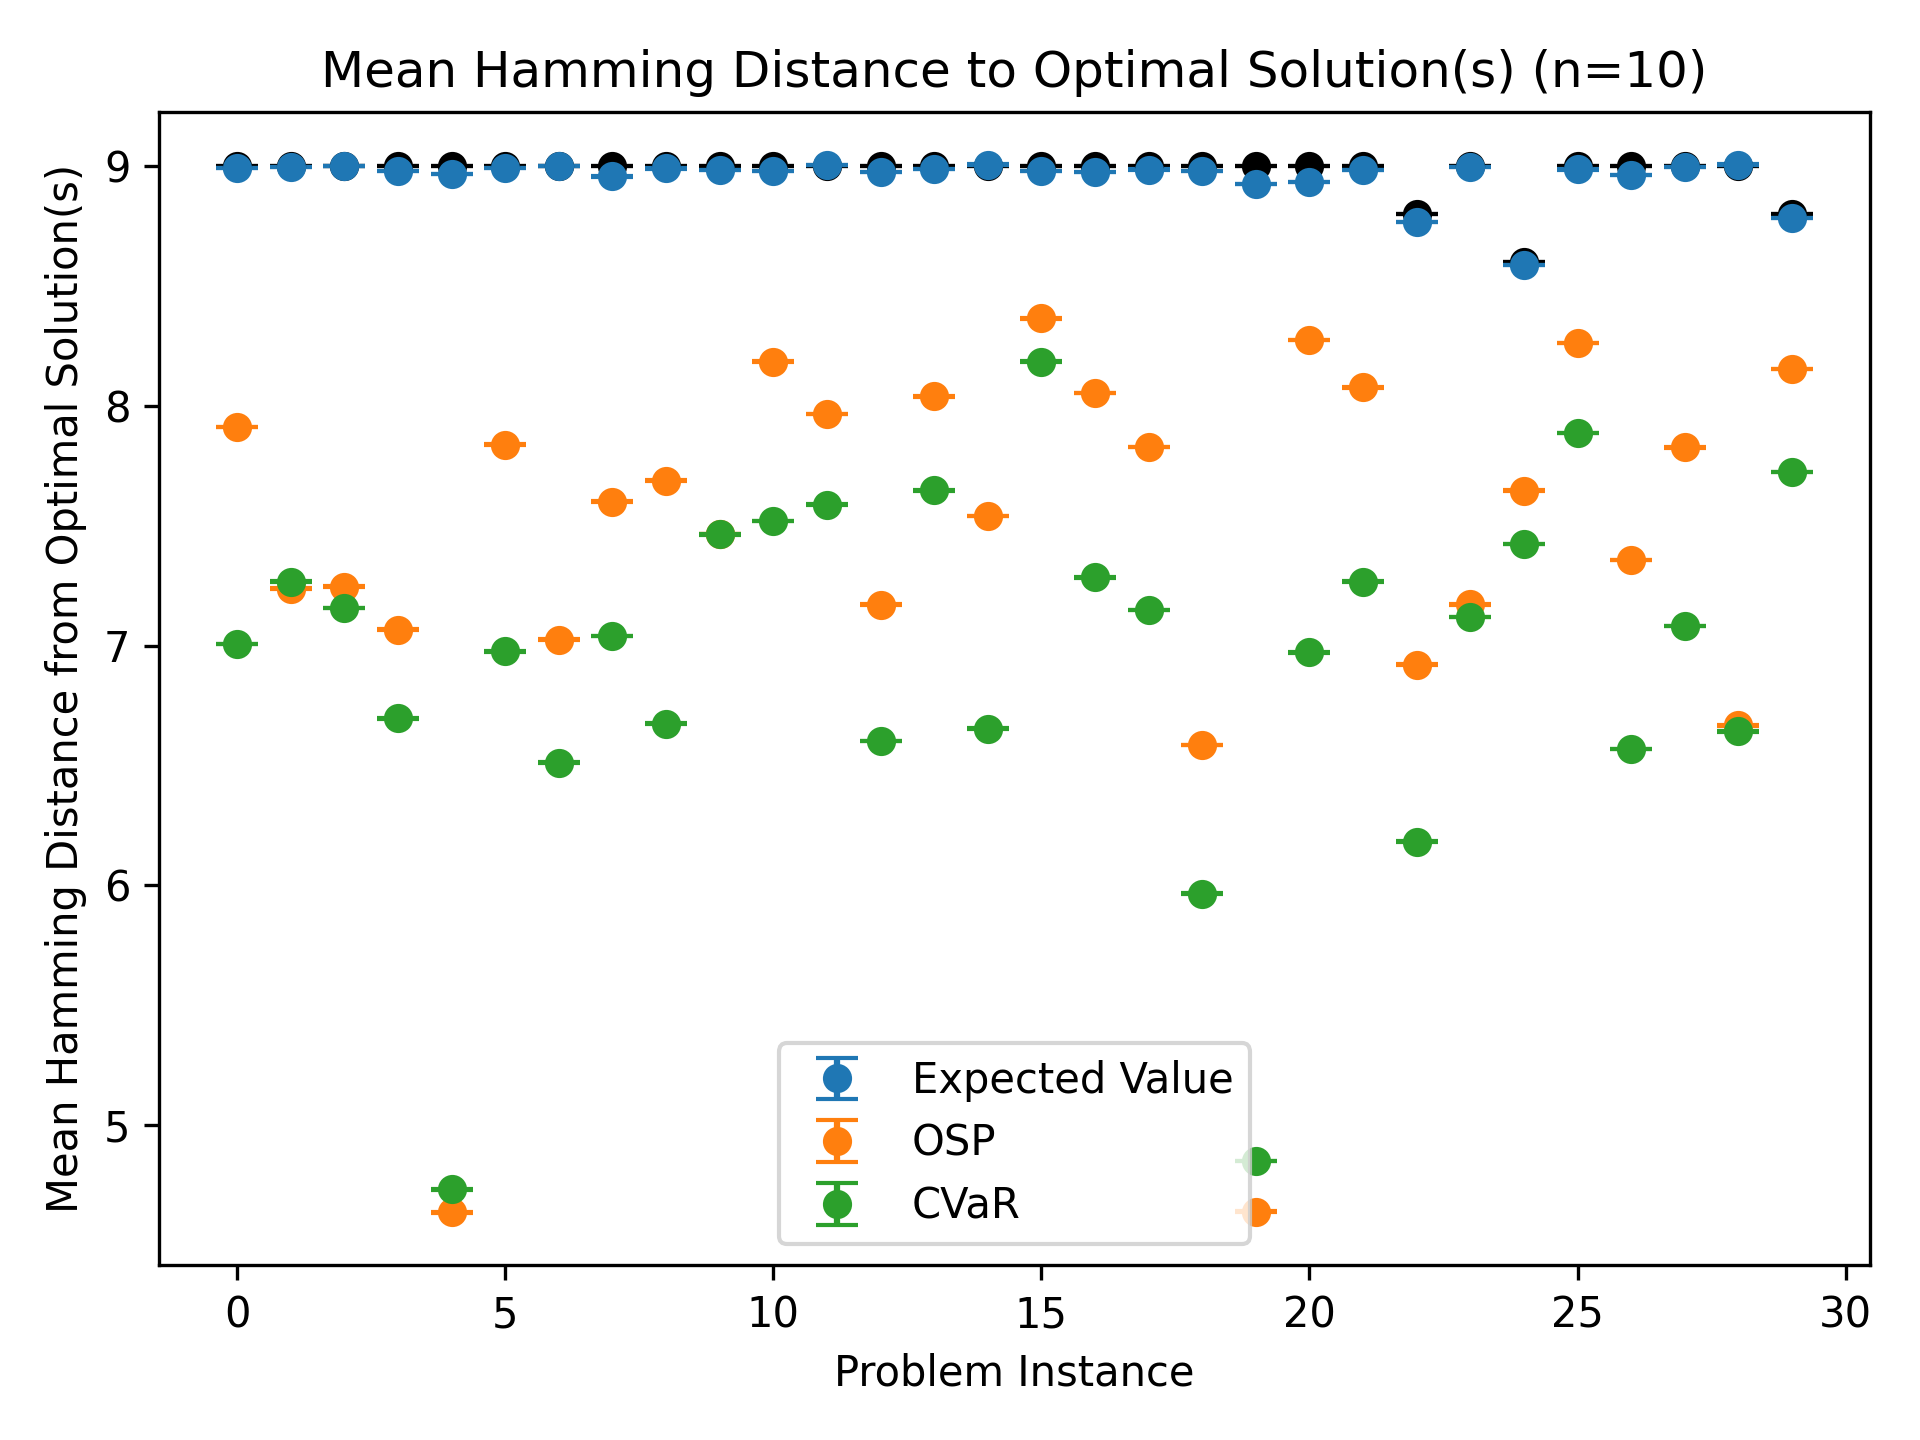
\includegraphics[width=\textwidth]{n=10_avg_hamming_distance_each_instance.png}
         \caption{$n=10$}
         \label{fig:avg ham 10}
     \end{subfigure}
        \caption{Mean hamming distance for each problem instance.}
        \label{fig:avg ham}
\end{figure}

As shown in Figure \ref{fig:ham improvement}, the mean Hamming distance decreased significantly after amplification, with X and Y and Z as the average reductions.
\begin{figure}[htbp]
    \centering
    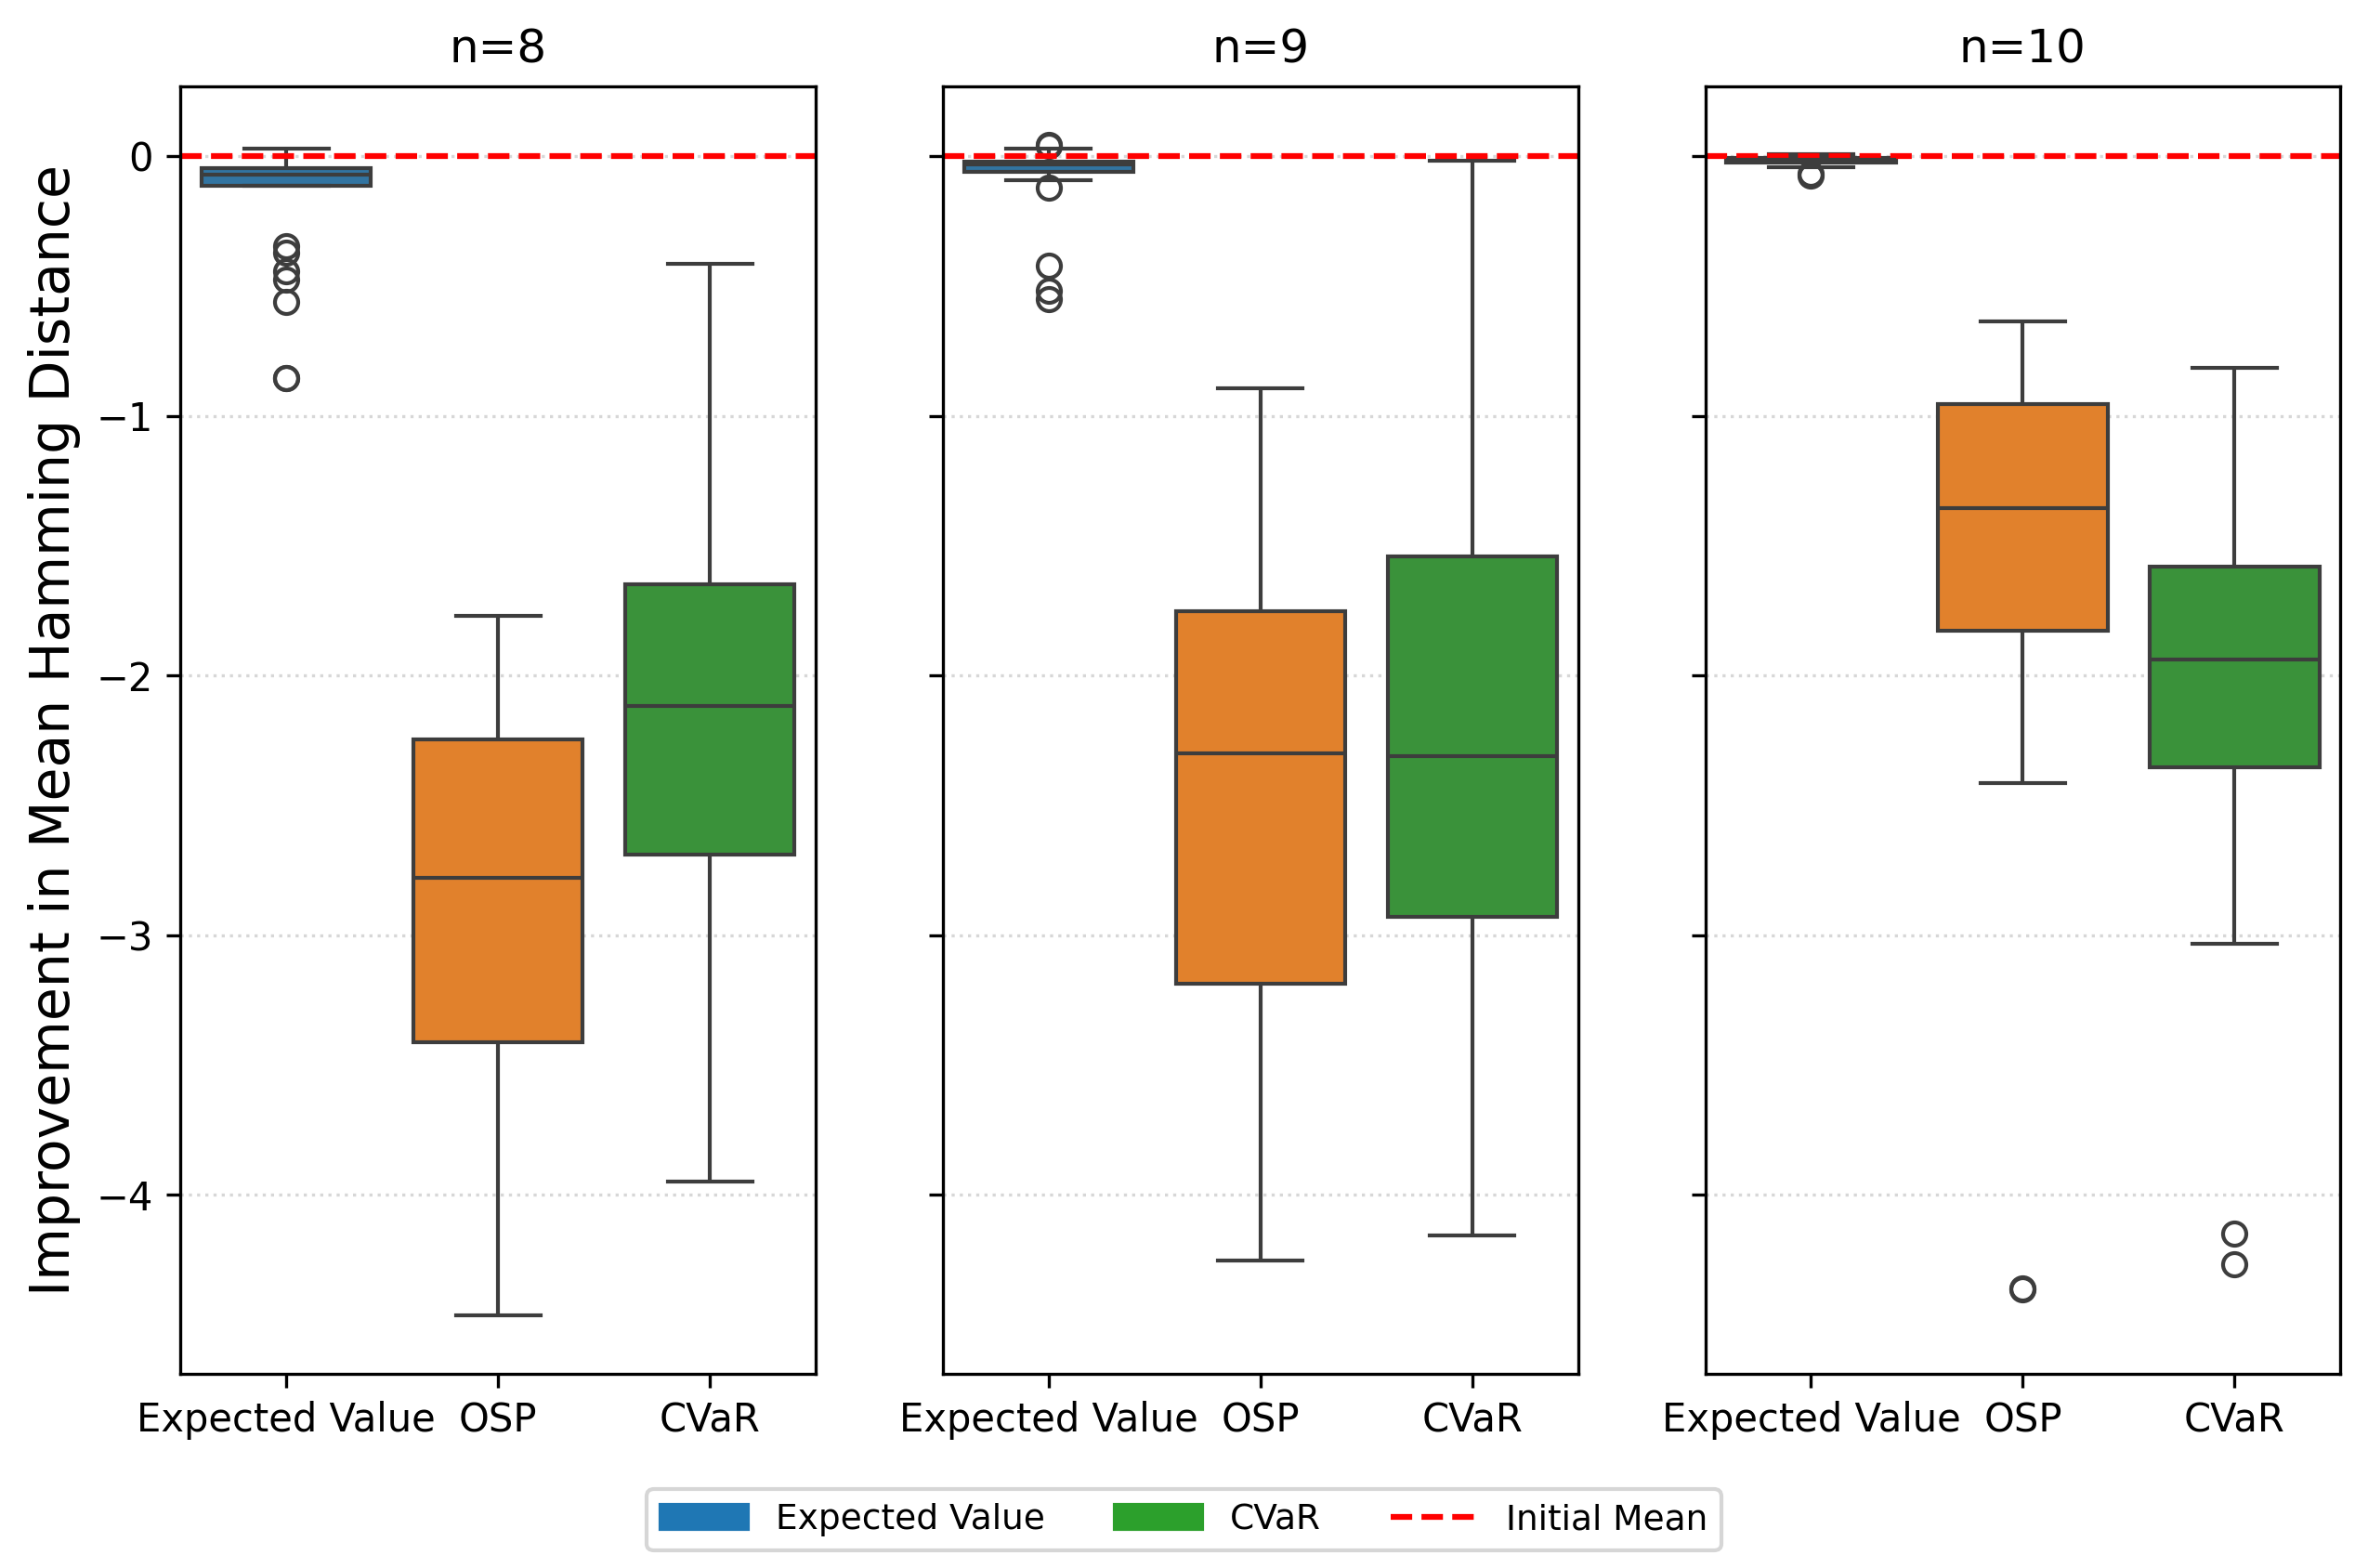
\includegraphics[width=\textwidth]{hamming_improvement_boxplot_multiple.png}
    \caption{Improvement in Hamming distance. This shows the change in expected Hamming distance after applying the NVQWOA for $p=10$ iterations.}
    \label{fig:ham improvement}
\end{figure}

Figure \ref{fig:amp vs ham} shows how much amplification was applied to each solution based on their Hamming distance. The optimal solutions received average amplifications of X,Y and Z.
\begin{figure}[htbp]
    \centering
    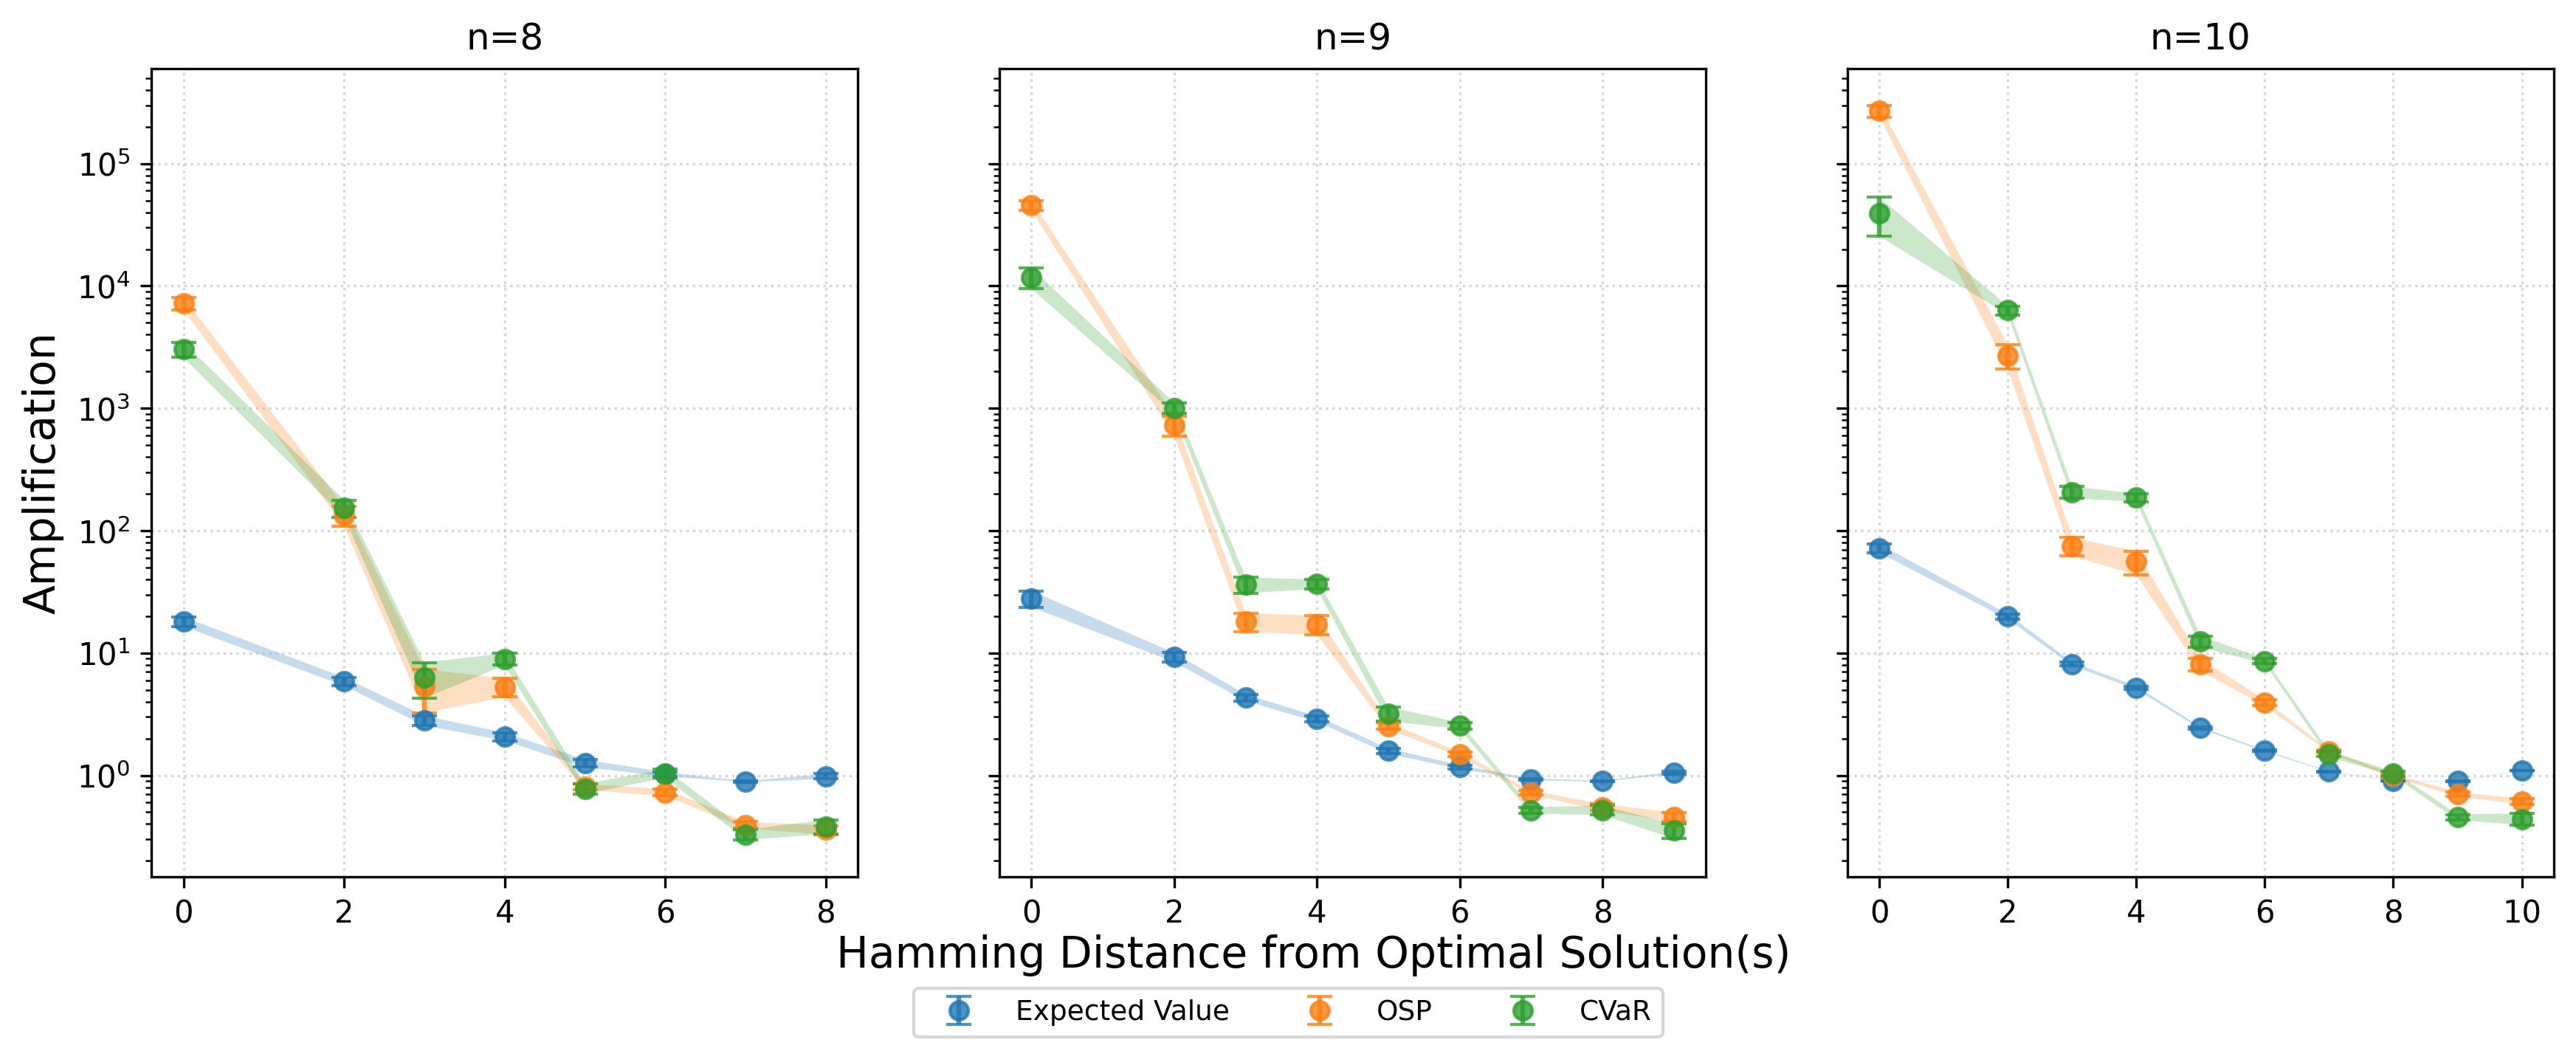
\includegraphics[width=\textwidth]{amplification_vs_hamming_multiple.png}
    \caption{Mean amplification applied to each solution grouped by their Hamming distance from the optimal solution.}
    \label{fig:amp vs ham}
\end{figure}

\section{Subshell Distance Analysis}
We also analysed the subshell distance between each solution and the optimal solution(s), which directly reflects the structure of the permutation mixer and the connectivity of the mixing graph.

Figure \ref{fig:avg sub} depicts the average subshell distance before and after amplification for each problem instance.
\begin{figure}[htbp]
     \centering
     \begin{subfigure}{0.45\textwidth}
         \centering
         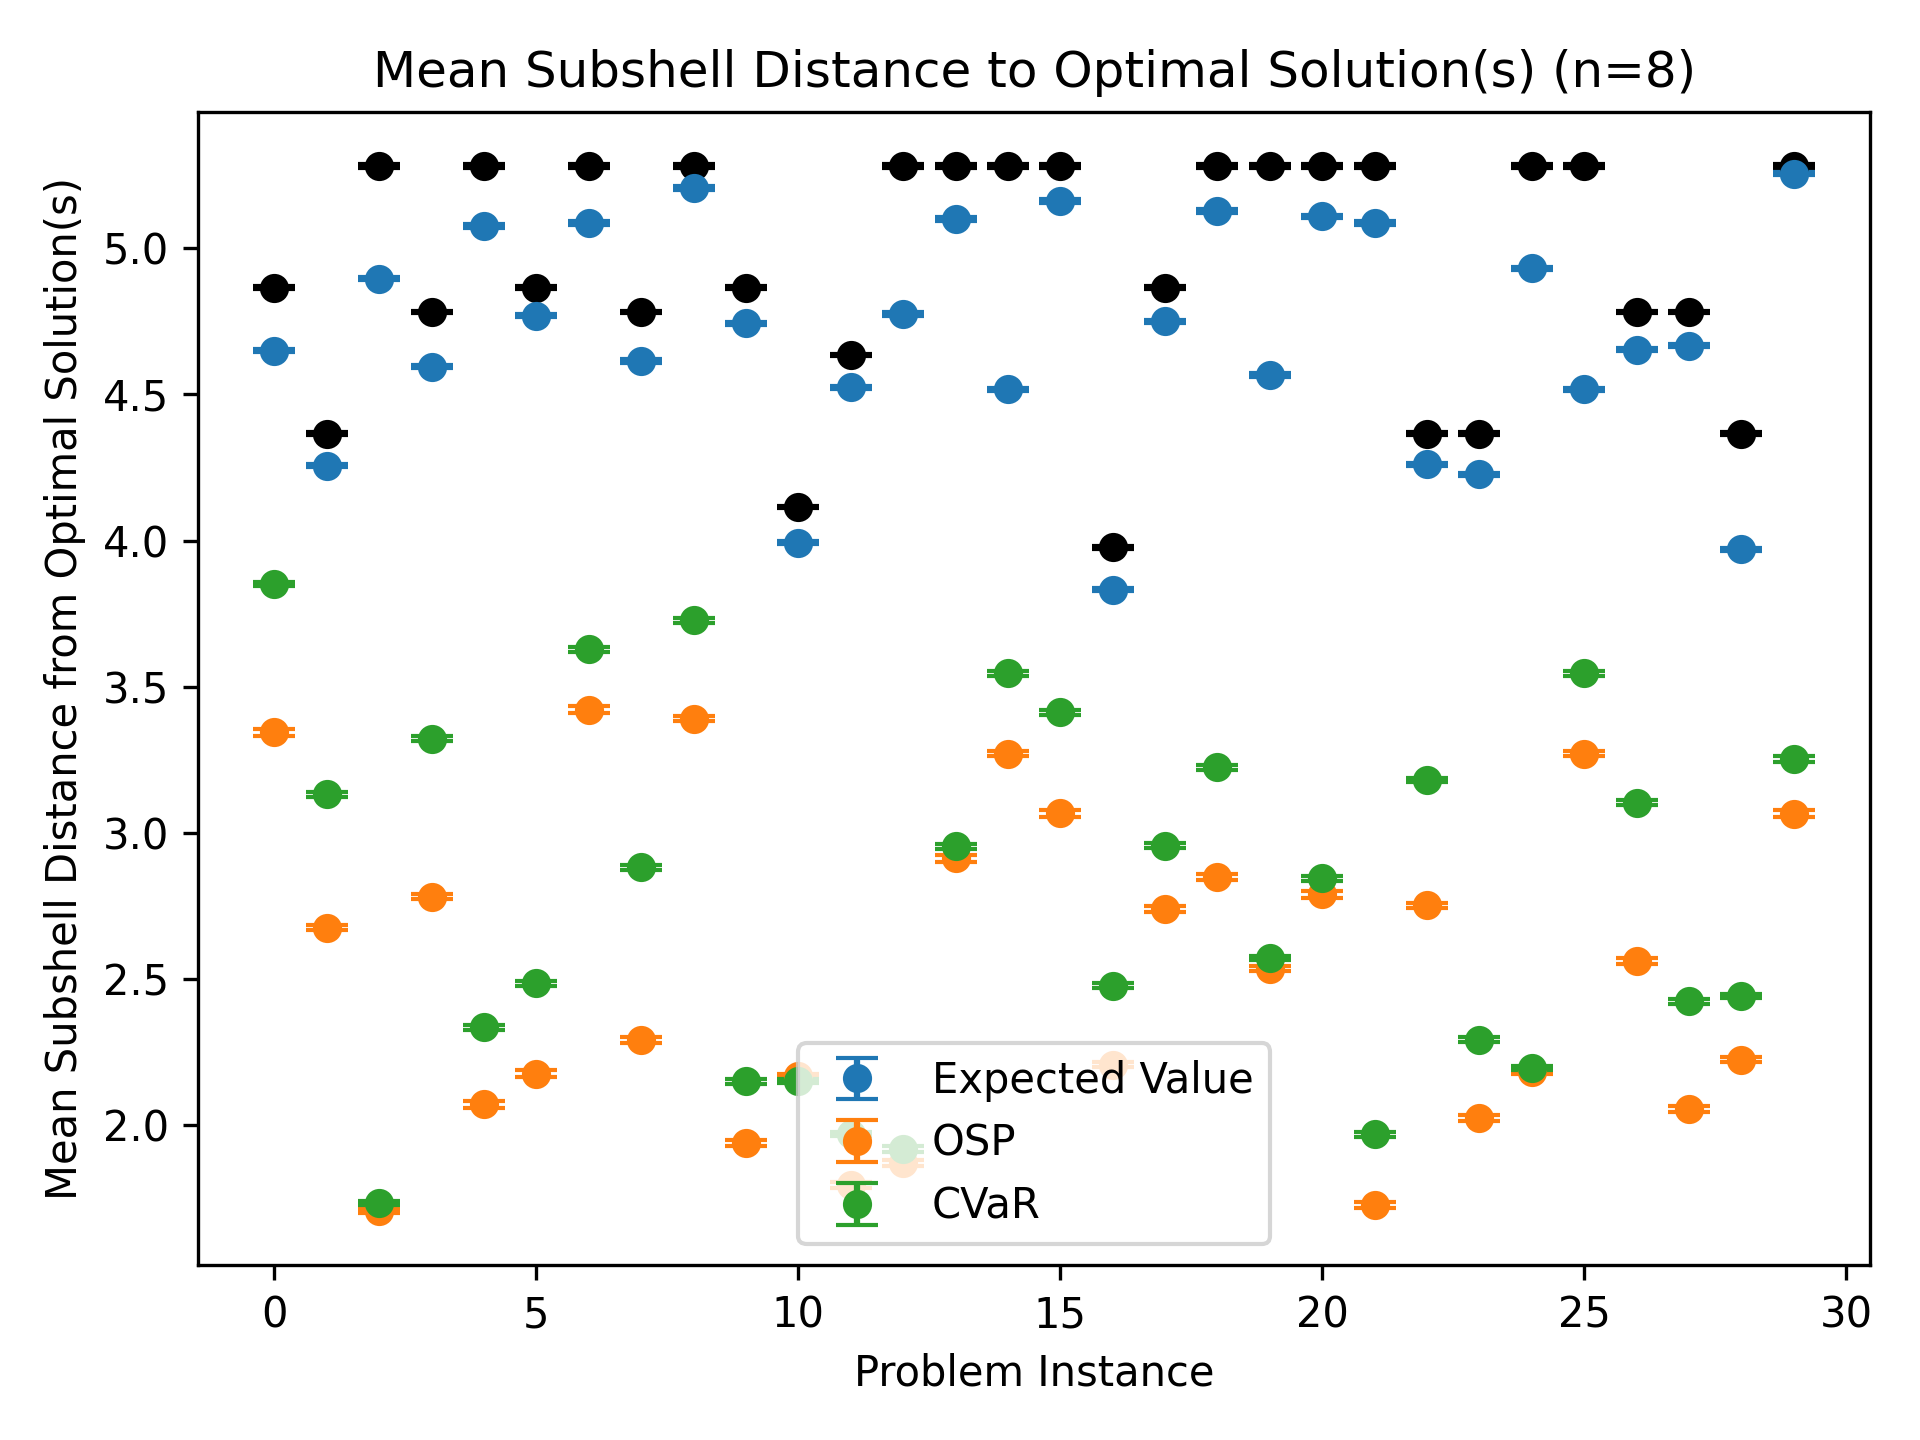
\includegraphics[width=\textwidth]{n=8_avg_subshell_distance_each_instance.png}
         \caption{$n=8$}
         \label{fig:avg sub 8}
     \end{subfigure}
     \hfill
     \begin{subfigure}{0.45\textwidth}
         \centering
         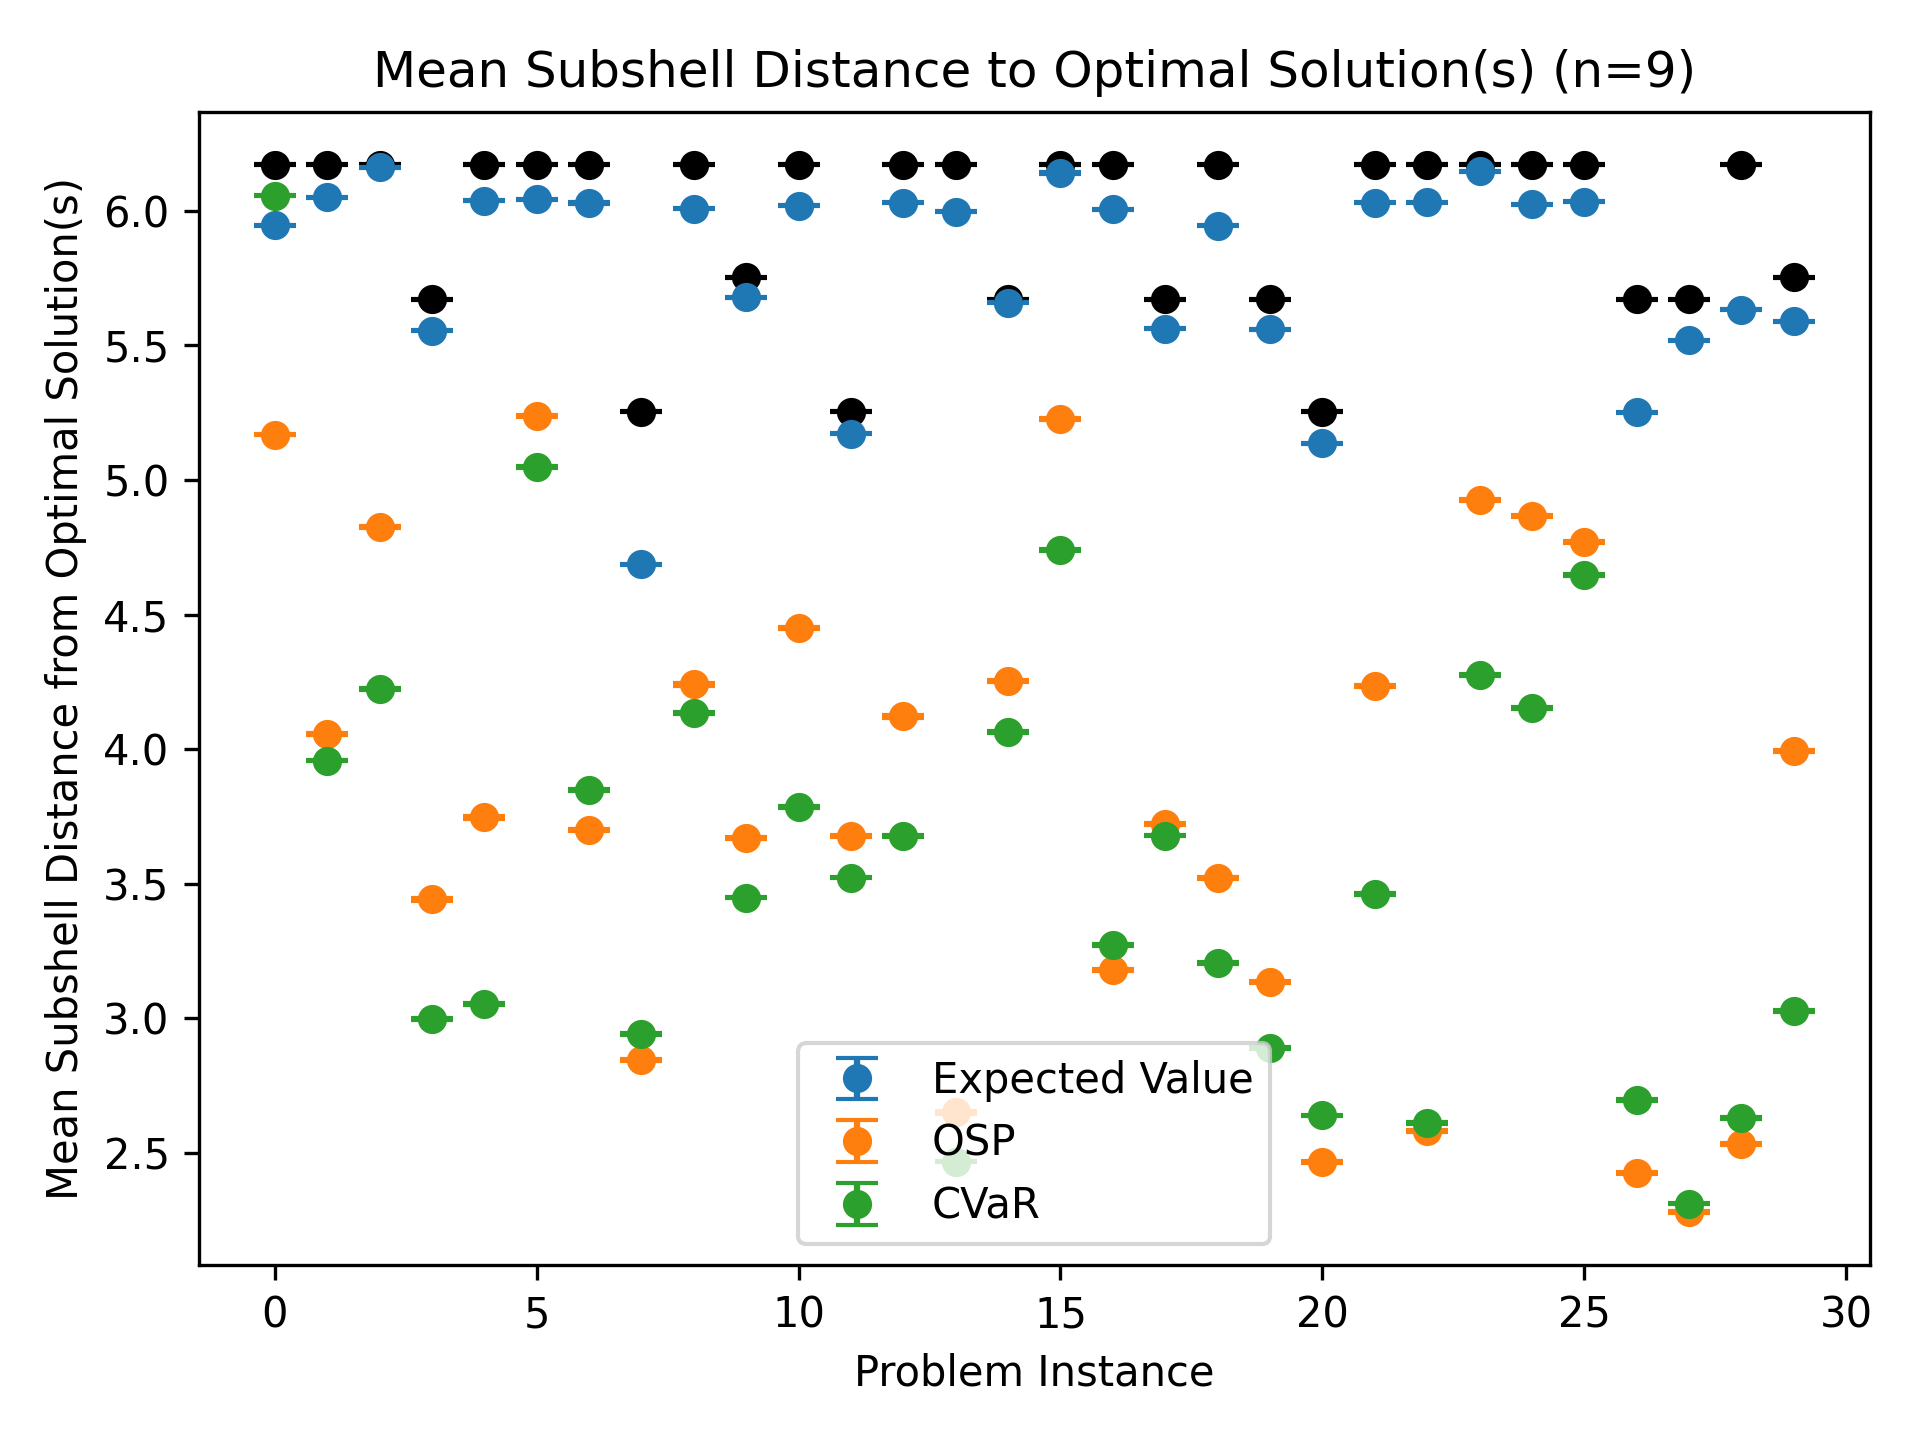
\includegraphics[width=\textwidth]{n=9_avg_subshell_distance_each_instance.png}
         \caption{$n=9$}
         \label{fig:avg sub 9}
     \end{subfigure}
     \hfill
     \begin{subfigure}{\textwidth}
         \centering
         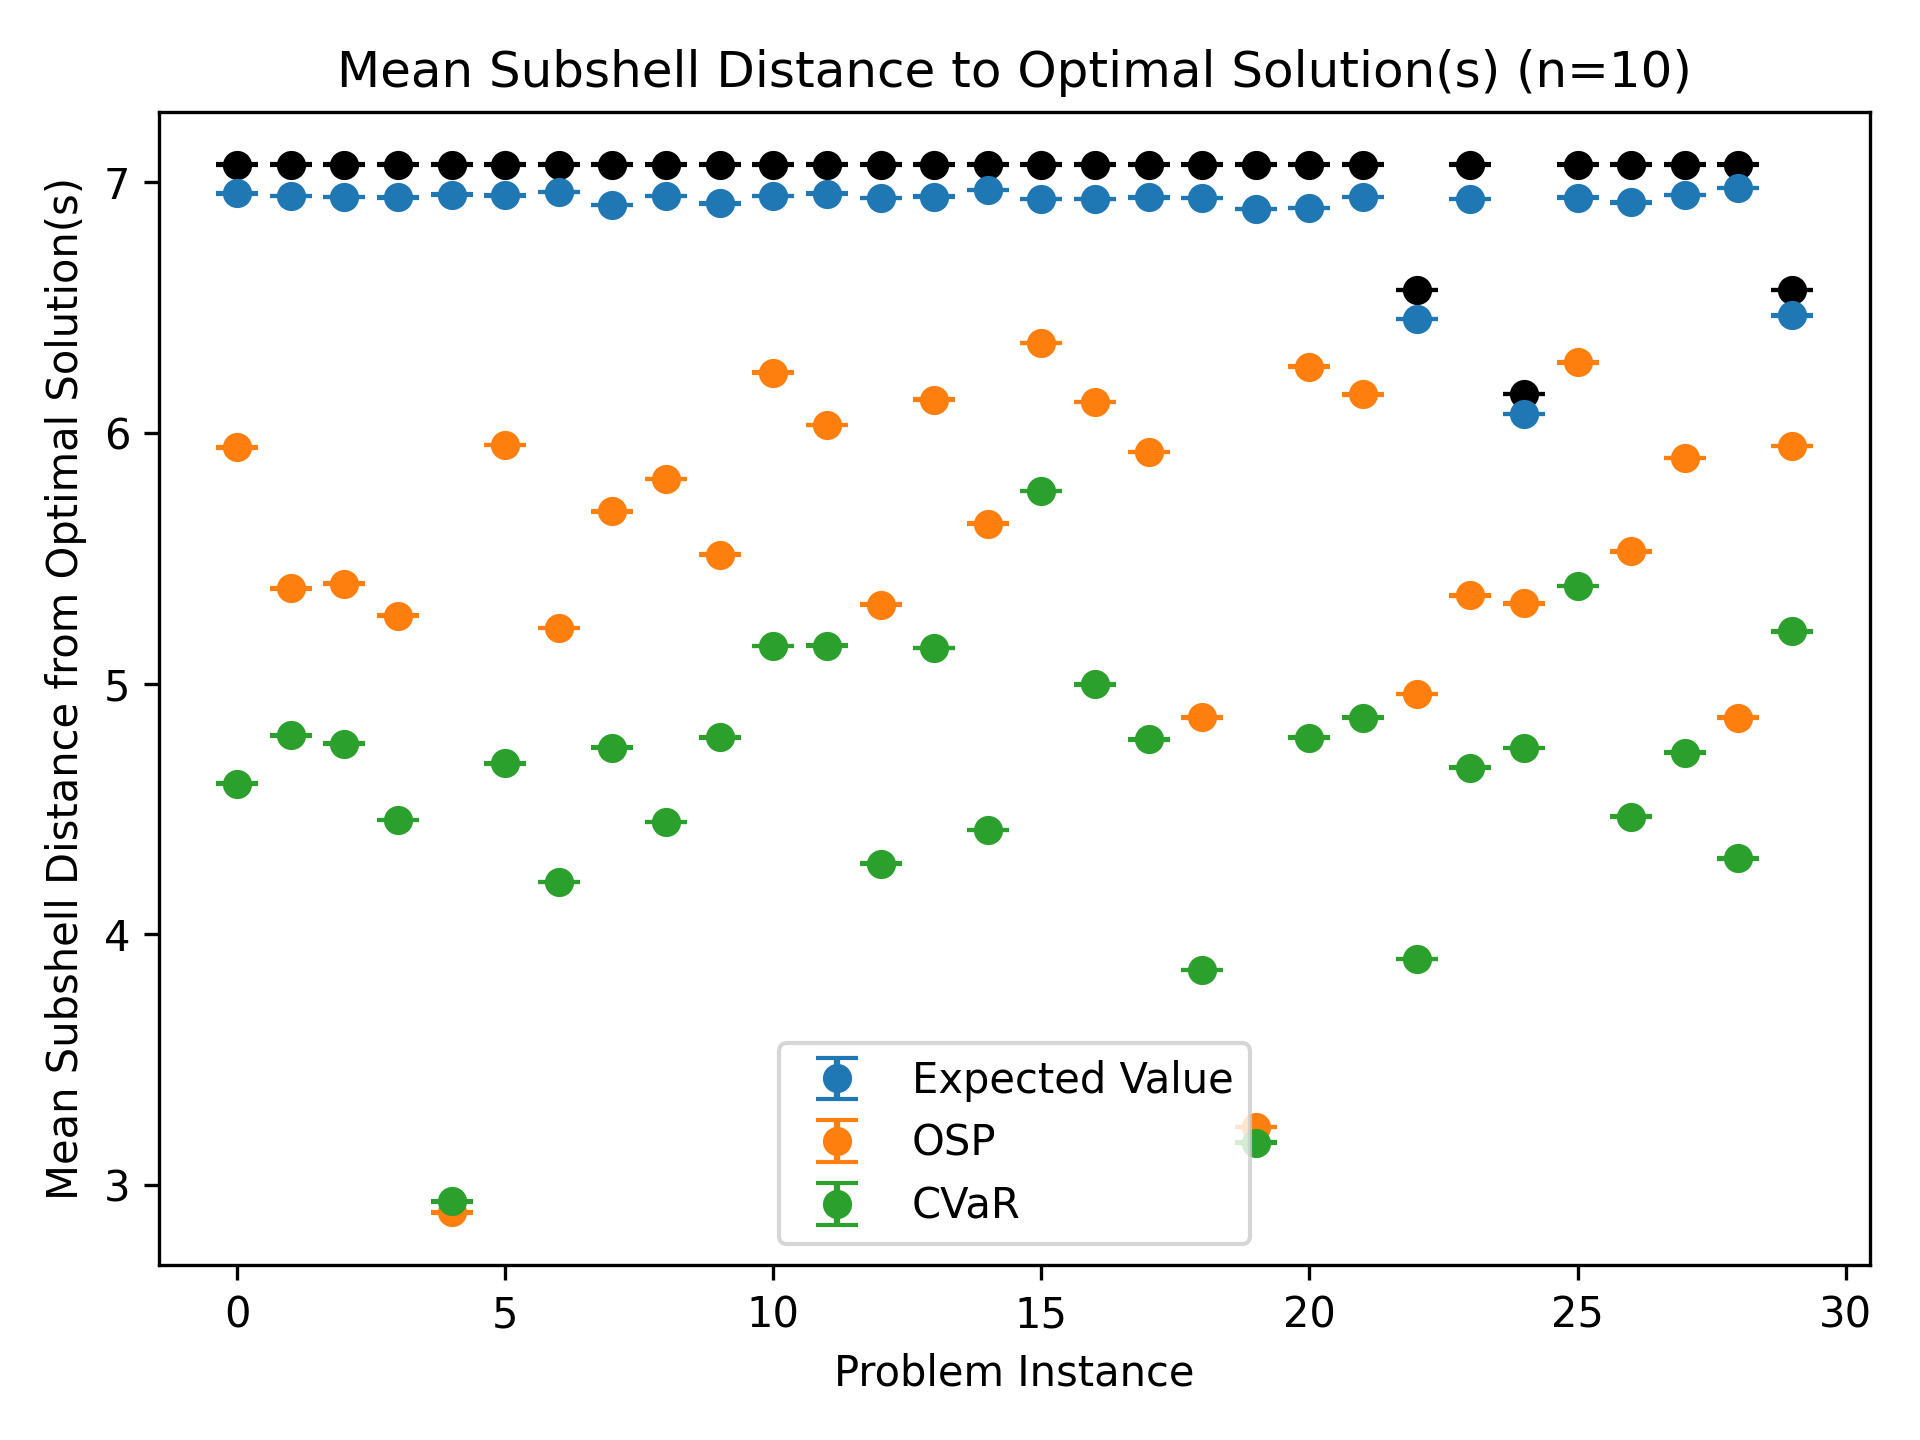
\includegraphics[width=\textwidth]{n=10_avg_subshell_distance_each_instance.png}
         \caption{$n=10$}
         \label{fig:avg sub 10}
     \end{subfigure}
        \caption{Mean subshell distance for each problem instance.}
        \label{fig:avg sub}
\end{figure}

Figure \ref{fig:sub improvement} shows the difference in mean subshell distance after amplification.
\begin{figure}[htbp]
    \centering
    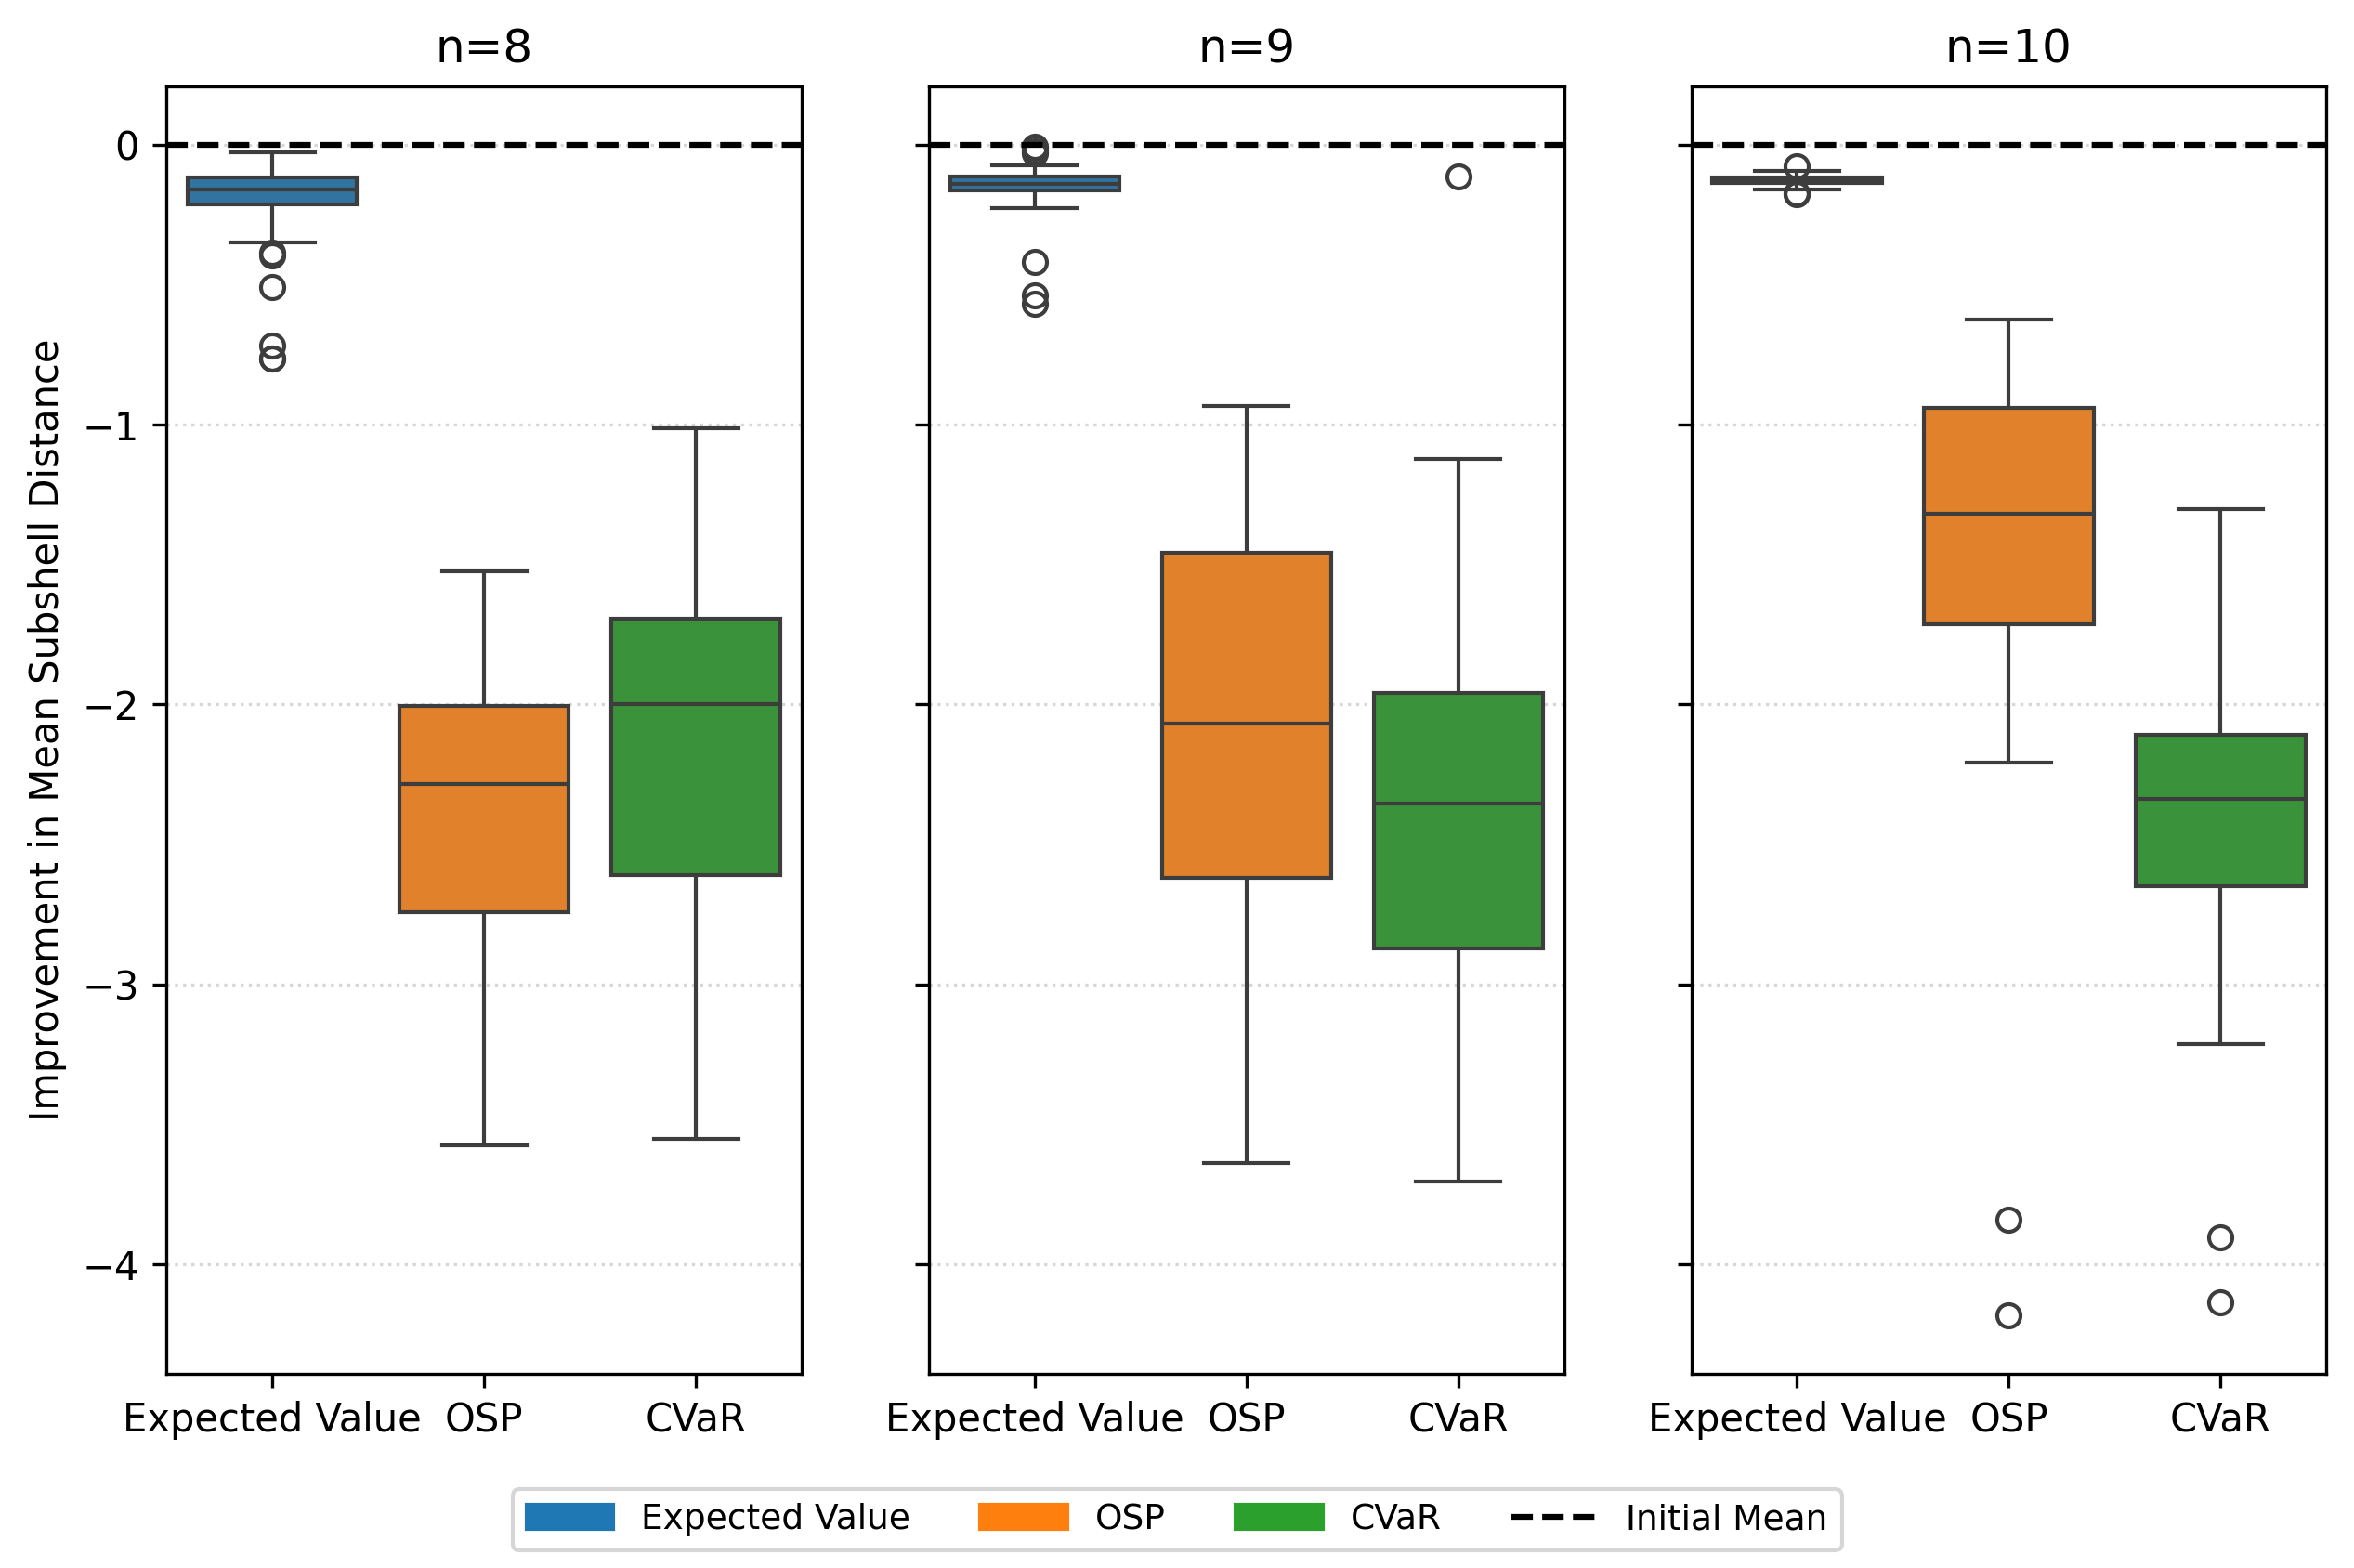
\includegraphics[width=\textwidth]{subshell_improvement_boxplot_multiple.png}
    \caption{Improvement in subshell distance boxplot.}
    \label{fig:sub improvement}
\end{figure}

Figure \ref{fig:amp vs sub} shows how much amplification was applied to each solution based on their subshell distance. These plots are monotonically decreasing. 
\begin{figure}[htbp]
    \centering
    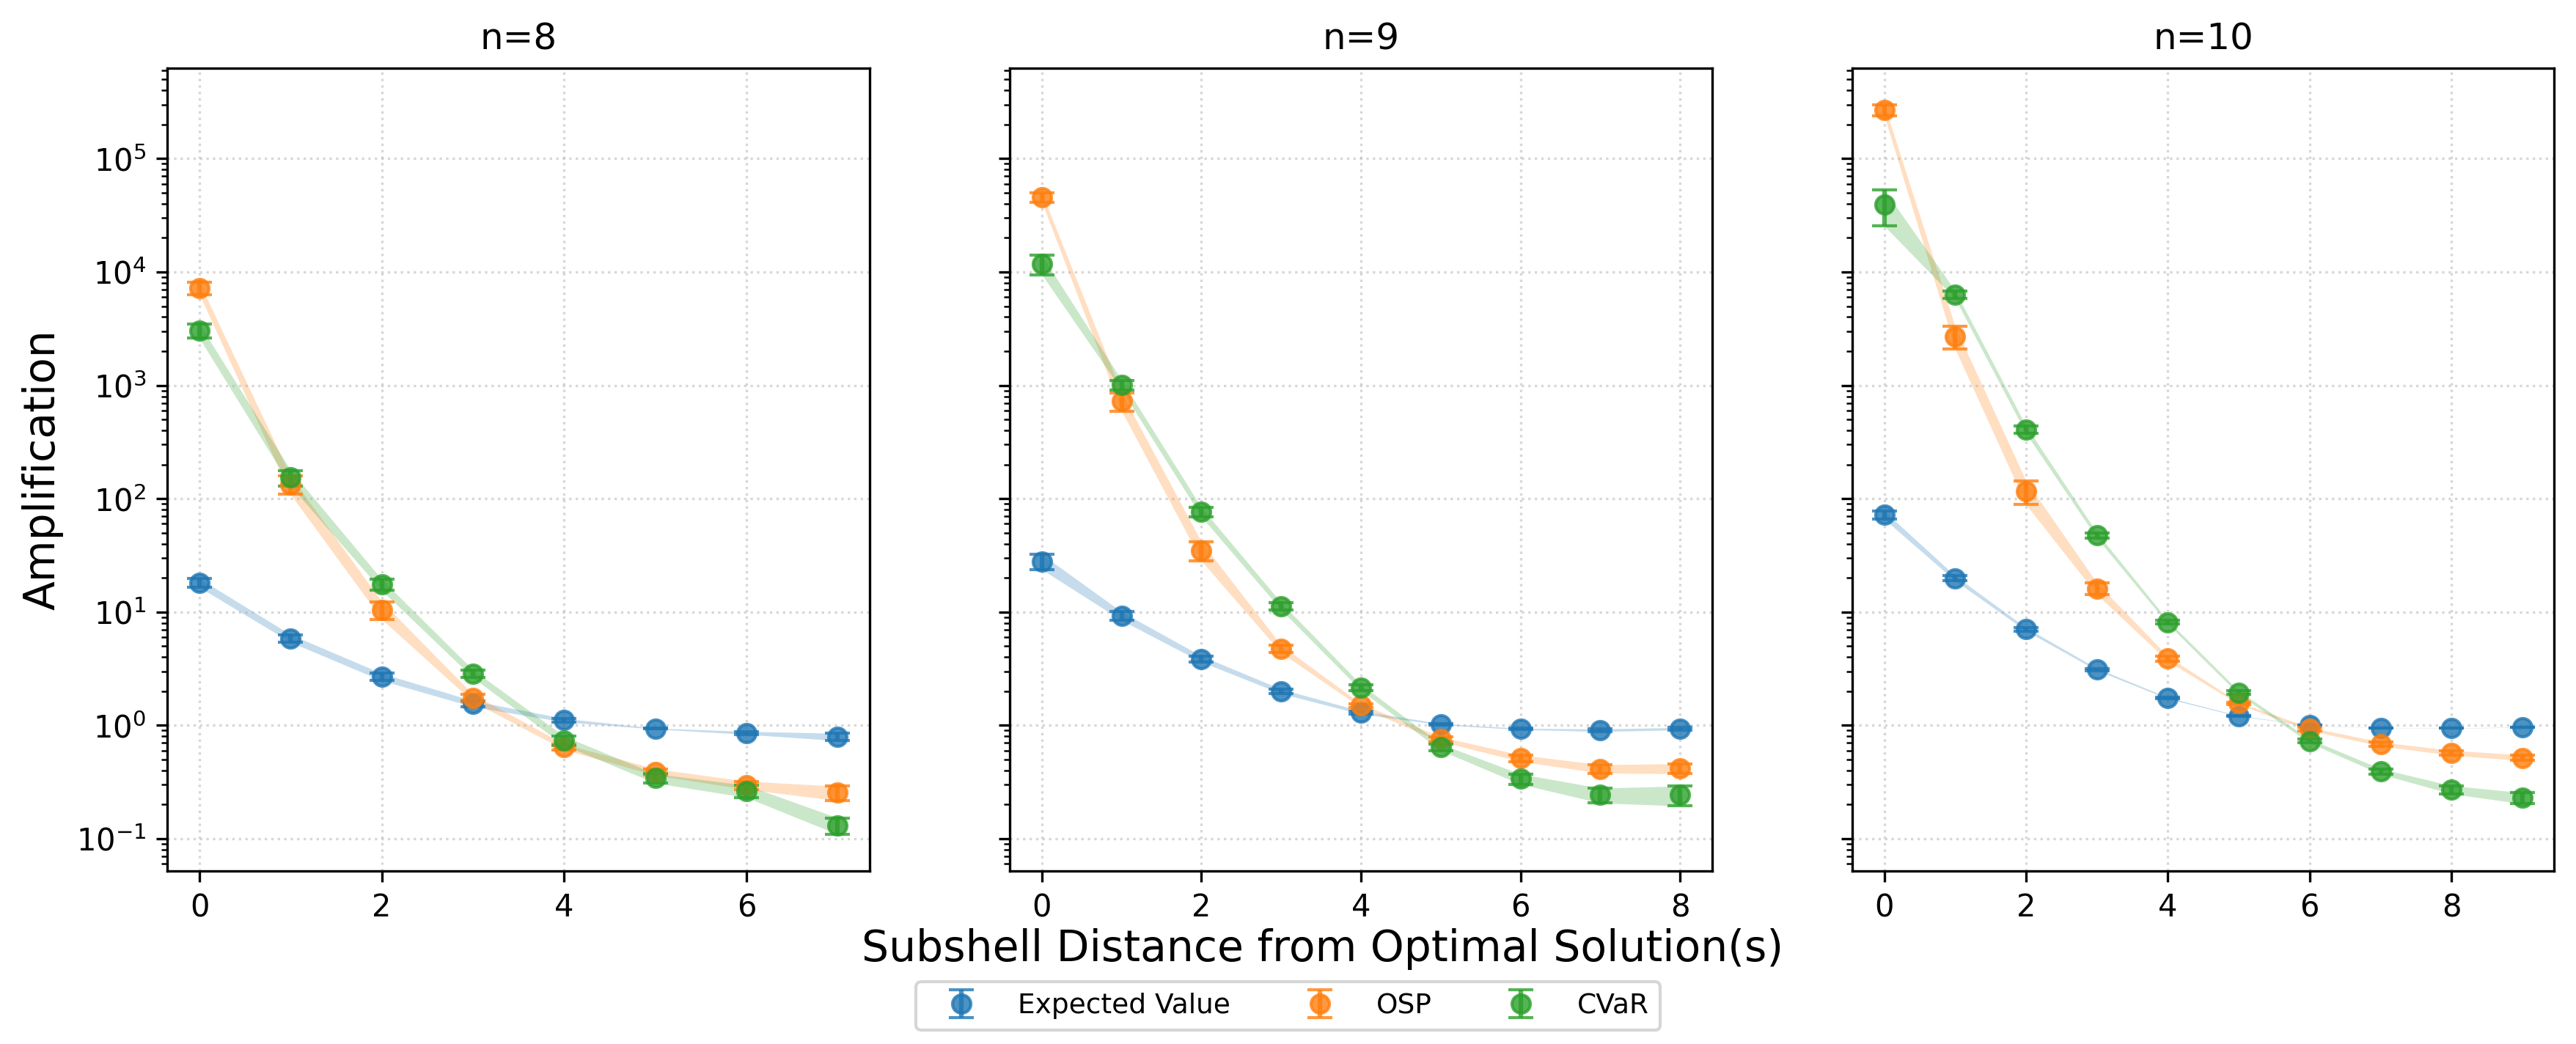
\includegraphics[width=\textwidth]{amplification_vs_subshell_multiple.png}
    \caption{Mean amplification applied to each solution grouped by their subshell distance from the optimal solution.}
    \label{fig:amp vs sub}
\end{figure}

Figure \ref{fig:mqg} shows the mean quality gap between the optimal solutions and the subshells. For all problem instances, the mean quality gap was a monotonically increasing function with subshell distance.
\begin{figure}[htbp]
    \centering
    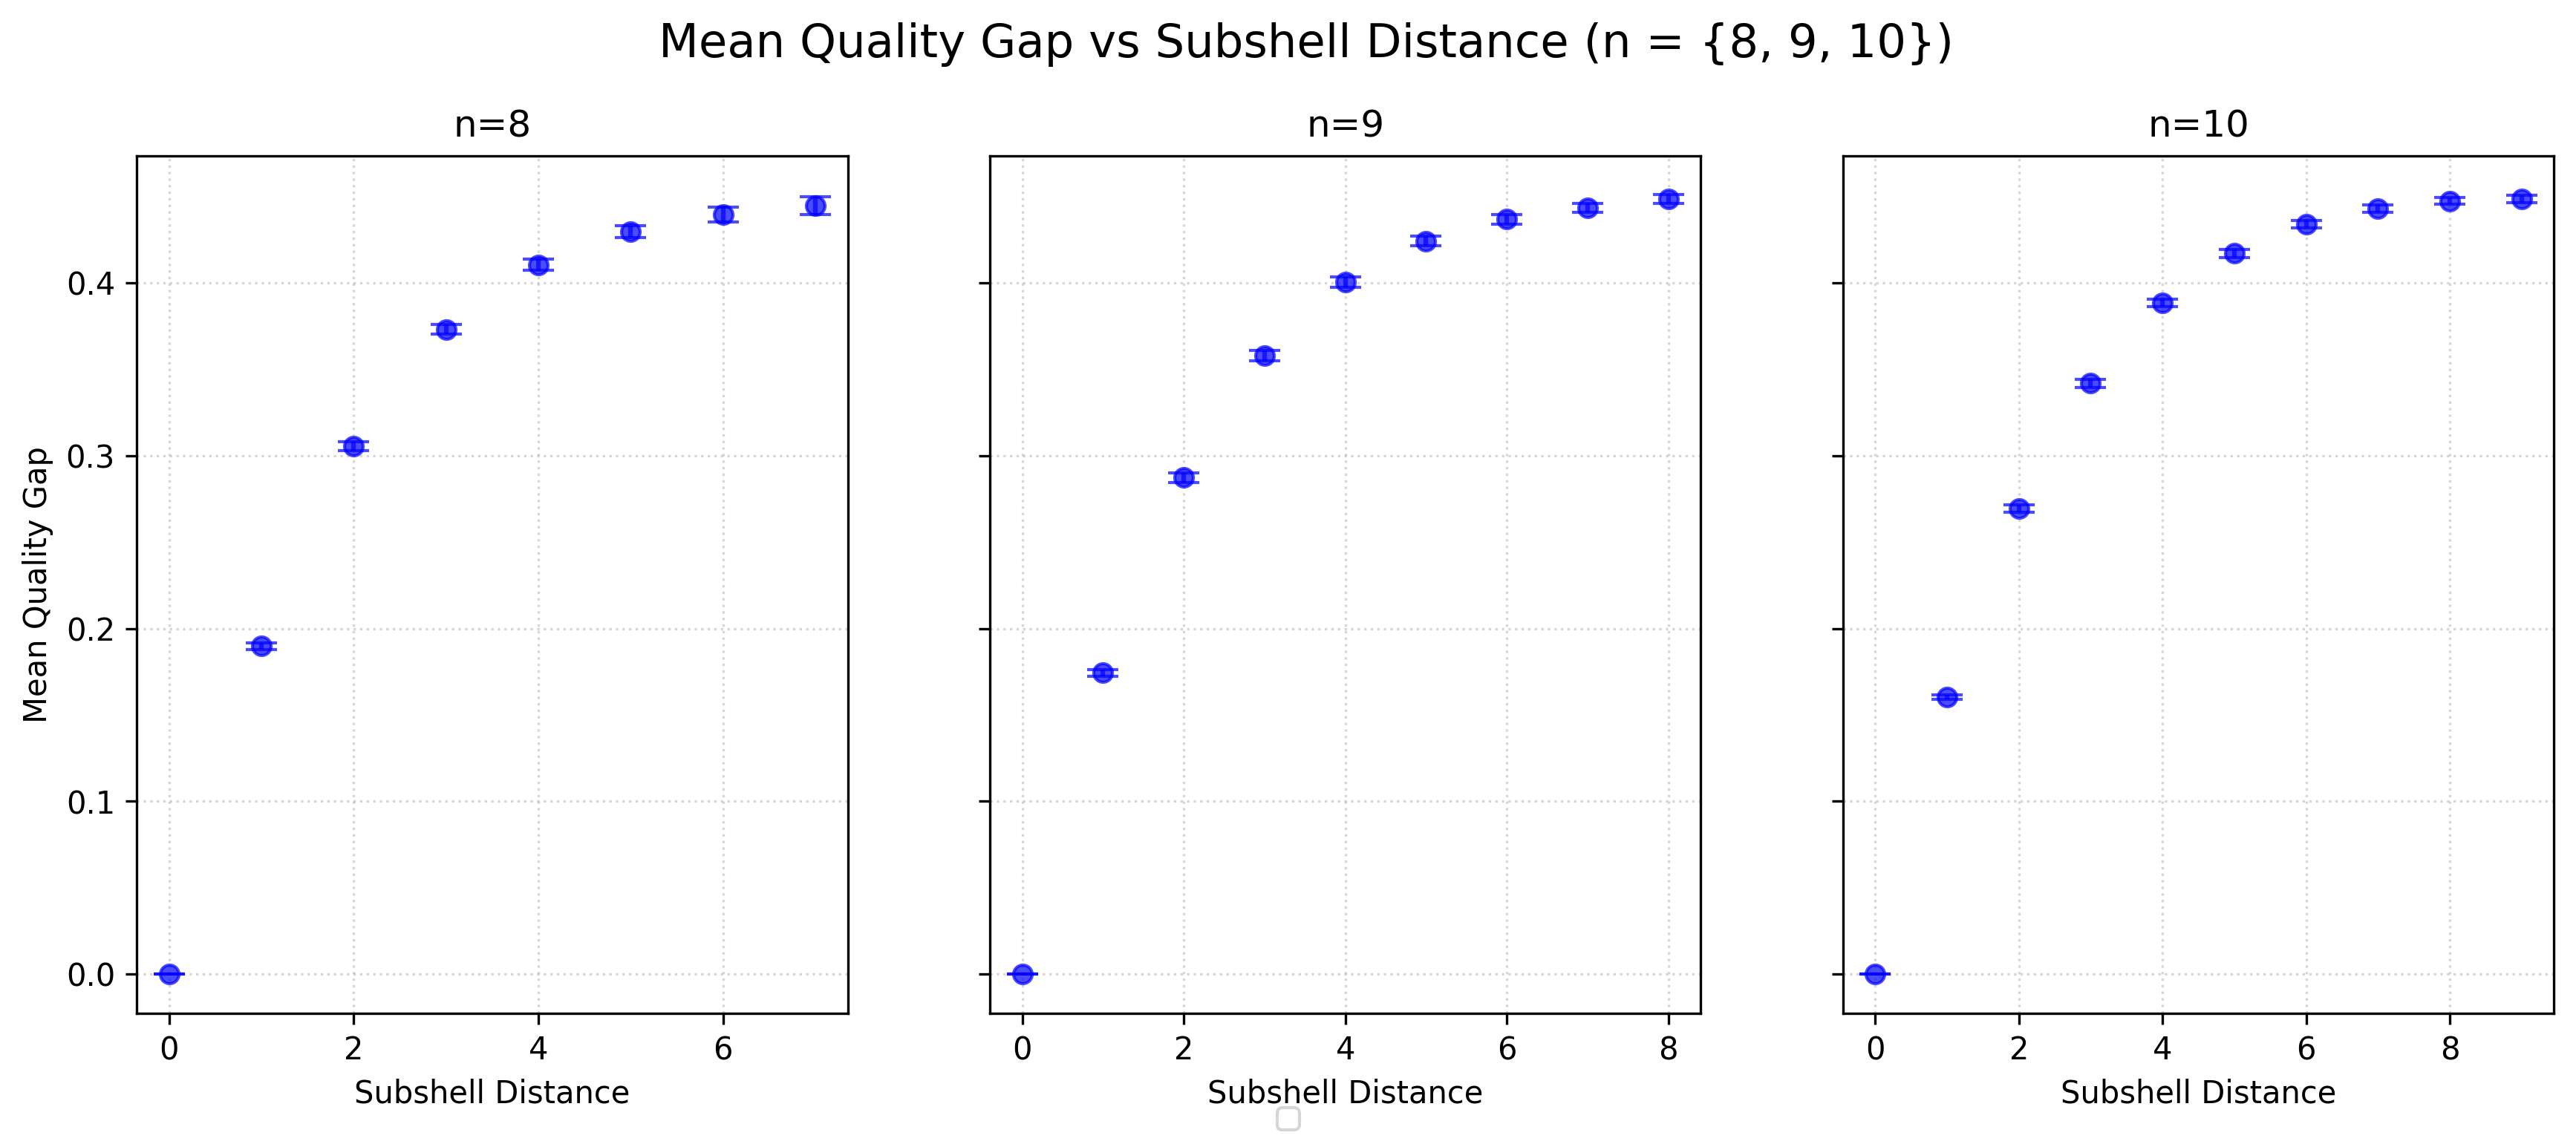
\includegraphics[width=\textwidth]{mean_quality_gap_vs_subshell_distance.png}
    \caption{Mean quality gap vs subshell distance}
    \label{fig:mqg}
\end{figure}

Figure \ref{fig:shell variance} shows the amount of variance in the objective values for each subshell.
Lower variance indicates more phase-coherence within the shell, and therefore more potential for constructive interference with the target solution under optimisation of $t$ and $\gamma$. The maximum subshell variance was X, for subshell $h$ in problem $k$.\todo{find max variance}
\begin{figure}[htbp]
    \centering
    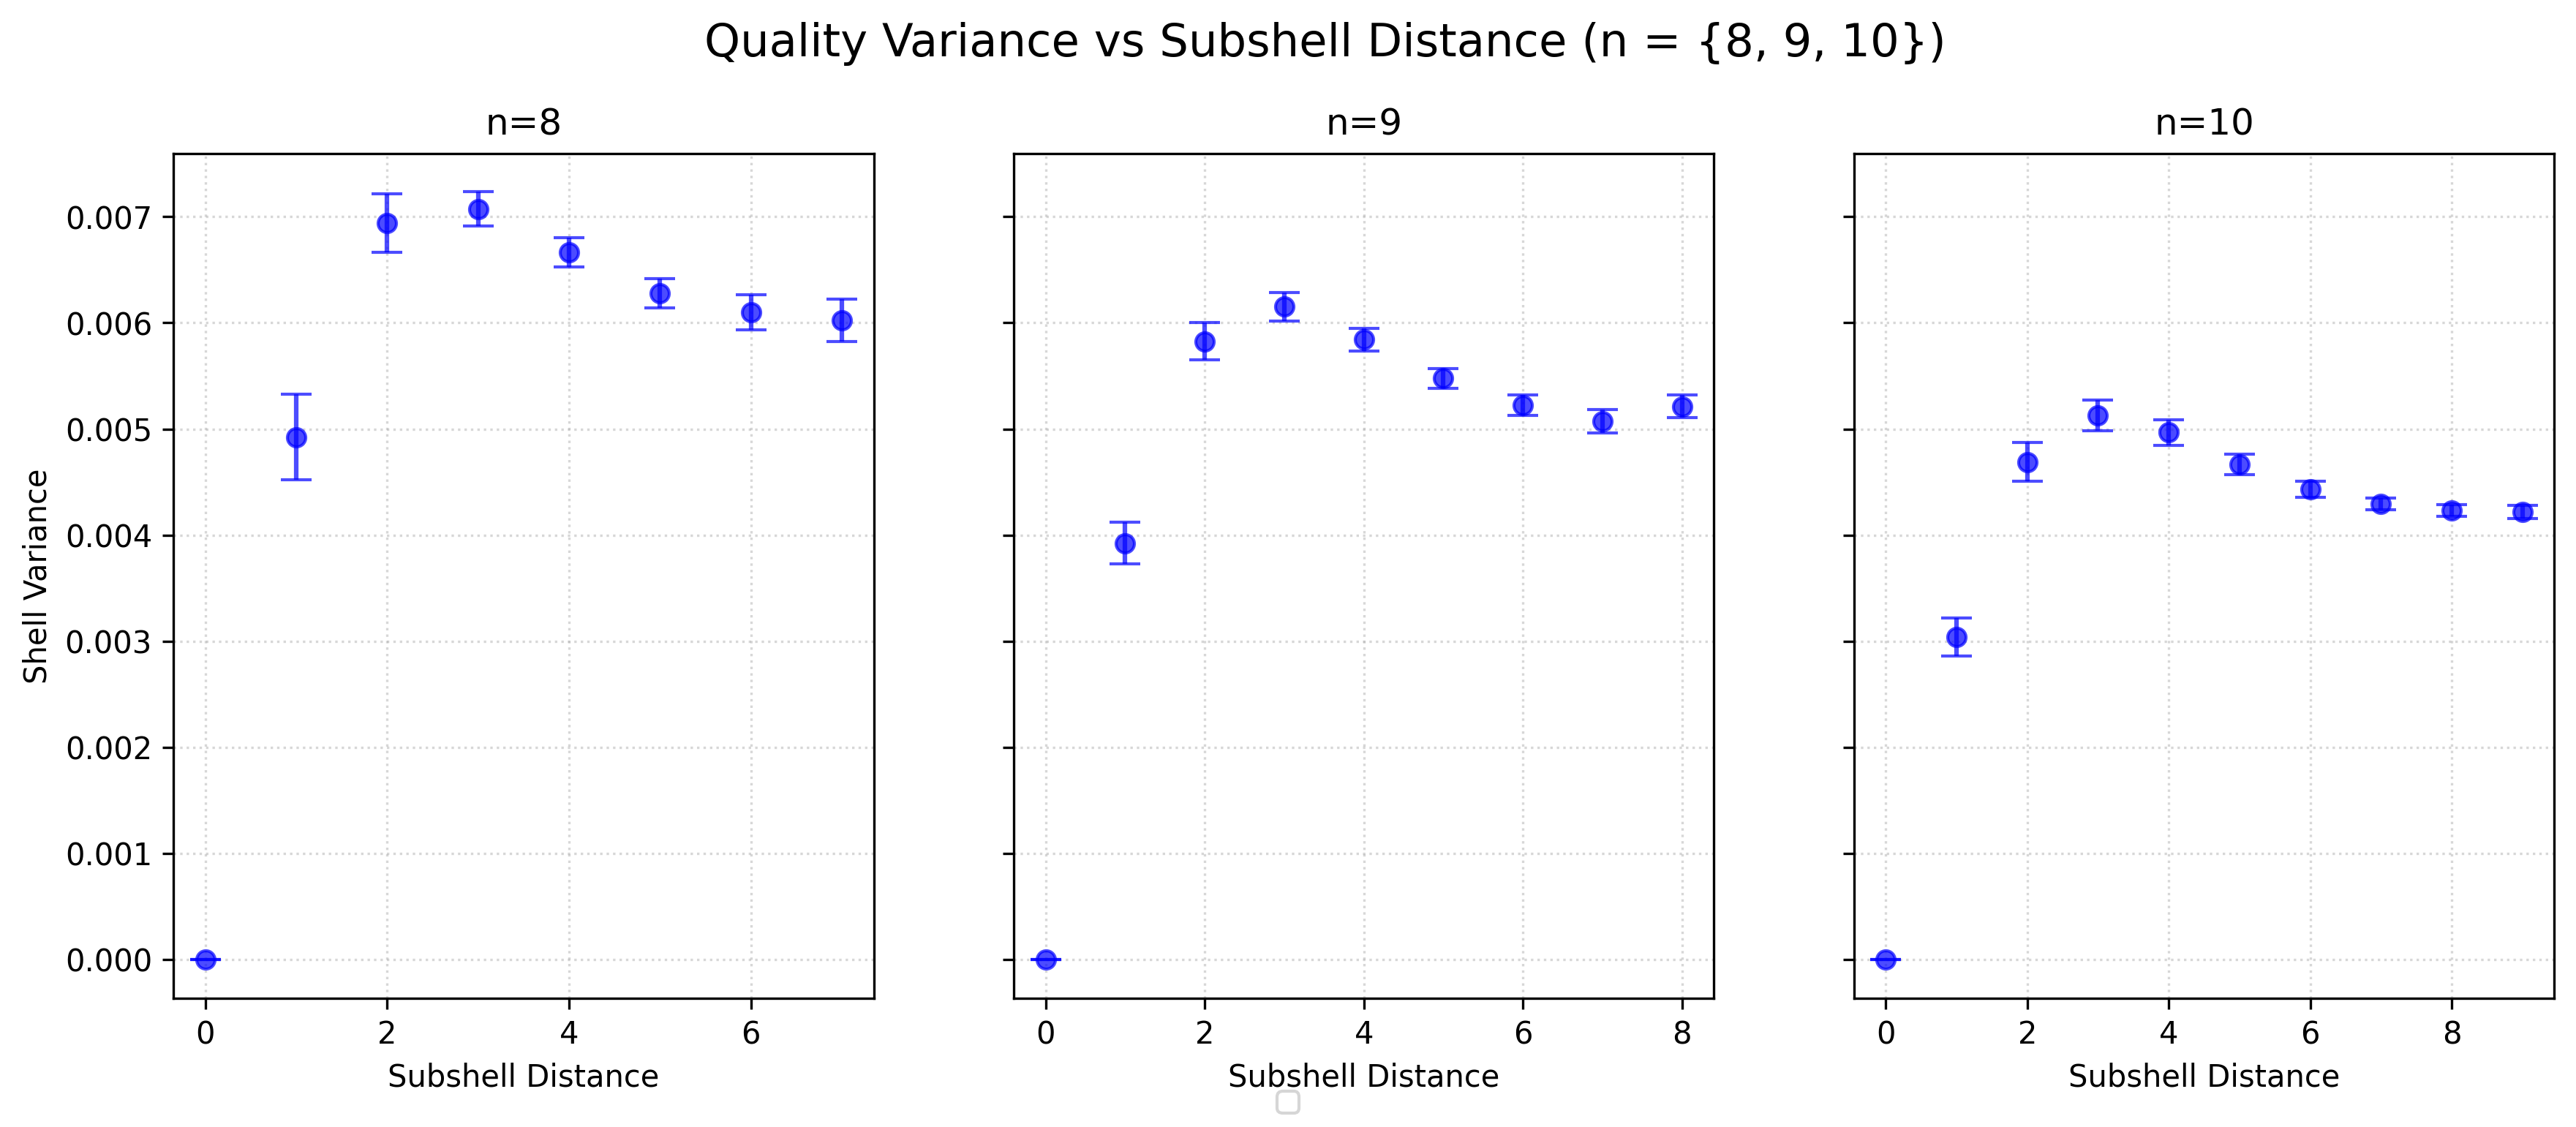
\includegraphics[width=\textwidth]{subshell_variance_multiple.png}
    \caption{Shell variance vs subshell distance}
    \label{fig:shell variance}
\end{figure}

\section{Hyperparameter Analysis}
We optimised the three NVQWOA hyperparameters $\beta, \gamma, t$ under three different objective functions applied to the final state: the expected value (EV), the probability of measuring an optimal solution (OSP), and the conditional value at risk (CVaR).

Table of mean hyperparameters:

\begin{tabular}{c||l|l|l}
    $n=8$          & $\beta$ & $\gamma$ & $t$     \\\hline\hline
    EV & 0.50(4) & 0.25(2) & 0.470(8) \\\hline
    OSP & 0.20(2) & 0.94(2) & 0.75(2) \\\hline
    CVaR & 0.00(3) & 0.92(3) & 0.76(3) \\\hline
\end{tabular}

\begin{tabular}{c||l|l|l}
    $n=9$          & $\beta$ & $\gamma$ & $t$     \\\hline\hline
    EV & 0.48(2) & 0.235(7) & 0.50(1) \\\hline
    OSP & 0.20(1) & 1.03(3) & 0.67(2) \\\hline
    CVaR & 0.10(3) & 0.92(4) & 0.74(2) \\\hline
\end{tabular}

\begin{tabular}{c||l|l|l}
    $n=10$          & $\beta$ & $\gamma$ & $t$     \\\hline\hline
    EV & 0.36(1) & 0.297(6) & 0.520(7) \\\hline
    OSP & 0.185(6) & 1.12(2) & 0.58(1) \\\hline
    CVaR & 0.35(3) & 0.64(4) & 0.55(2) \\\hline
\end{tabular}
